\documentclass{my-article}
\usepackage{my-coverpage}

\usepackage[utf8]{inputenc}
\usepackage[T5]{fontenc}
\usepackage[vietnamese, english]{babel}

\usepackage{textcomp}
% =========================
% Cover page information
% =========================

\selectlanguage{vietnamese}
\NameUpperUniname{Vietnam National University Ho Chi Minh City}
\NameUniname{Ho Chi Minh City University of Technology}
\NameDeptname{Faculty of Electrical and Electronics Engineering}
\NamePathlogo{./my-chapters/my-images/01_logobachkhoatoi.png}
\NameClass{Digital signal processing on FPGA}
\NameGroup{08}
\NameLesson[\Large]{LABORATORY REPORT}
\NameTitle[\Huge]{Waveform generator}
\NameAdvisor{Nguyễn Tuấn Hùng}
\NamePlace{Ho Chi Minh}
\NameTime{../../20..}
\NamePathBackground[width=\paperwidth,height=\paperheight]{./my-chapters/my-images/bia.jpg} 
\MemberTableData{
1 & 2213874 & Nguyễn Thanh Tùng & L01 \\ \hline
2 & 2210780 & Nguyễn Đại Đồng & L01 \\ \hline
3 & 2213496 & Nguyễn Quốc Tín & L01 \\ \hline
}

% =========================
% Configuration
% =========================
%--- Header and footer
\fancyhf{}
\fancyhead[L]{\leftmark}
% =========================
% Document
% =========================
\begin{document}
\pagestyle{empty}
\MycoverFinalProject % Cover page
\newpage
\selectlanguage{english}
\renewcommand{\arraystretch}{1.5} % tăng khoảng cách dòng (row height)
\setlength{\parindent}{1cm}
\onehalfspacing
\setlength{\parskip}{6pt} 
\tableofcontents
\listoffigures
\listoftables
\newpage
\pagestyle{fancy}
\MycountPages{number}
\fancyfoot[L]{
\includegraphics[width=.02\linewidth]{./my-chapters/my-images/logo_DEE.png}\text{ Department of Electronics}}
\section{Introduction}

\subsection{Overview}

In the field of digital electronics and signal processing, FPGA (Field Programmable Gate Array) technology provides strong capabilities for high-speed and parallel execution of signal processing tasks. The topic\textbf{ “Design and Implementation of a Waveform Generator on the DE10 FPGA Kit”} is chosen with the main objective of creating a configurable test signal source, which is very important in digital signal processing experiments and applications.

The waveform generator is designed to produce signals with adjustable frequency, amplitude, and waveform type (such as sine, square, and triangle). This flexibility makes the system a reusable tool for testing and validating digital circuits and signal processing modules. In real engineering practice, having a programmable waveform generator on FPGA helps simulate real-world input signals and evaluate system performance under different conditions.

Implementing the waveform generator on FPGA also gives practical experience in hardware-level digital design. Students can apply knowledge of HDL programming (Verilog or VHDL), modular system design, and timing analysis. At the same time, they can practice functional verification of digital systems and learn how to combine theory with real hardware implementation.

This project not only strengthens understanding of digital signal processing concepts but also develops essential skills for embedded system and FPGA-based design careers.

\subsection{Assigned Objectives}

\begin{itemize}[label=-]
	\item Survey the hardware used in the project; read and study the datasheets of all selected components.
	\item Implement a top-level system architecture, then decompose it into modular blocks, each responsible for a specific function.
	\item Study the I²C protocol for WM8731 configuration and the I²S audio protocol for streaming audio data.
	\item Implement the waveform-generation logic for each waveform type, then provide run-time controls for amplitude, frequency, and duty cycle.
	\item Extend the system by injecting noise into the waveform.
	\item Develop comprehensive testbenches to verify and simulate each module’s functionality.
	\item Deploy and validate the design on the target development kit (hardware-in-the-loop) and confirm that measured results match simulation.
\end{itemize}
\section{Theoretical Background}

\subsection{Introduction of the DE10-Standard Board}

\subsubsection{Layout and Components}

\begin{figure}[H]
	\centering
	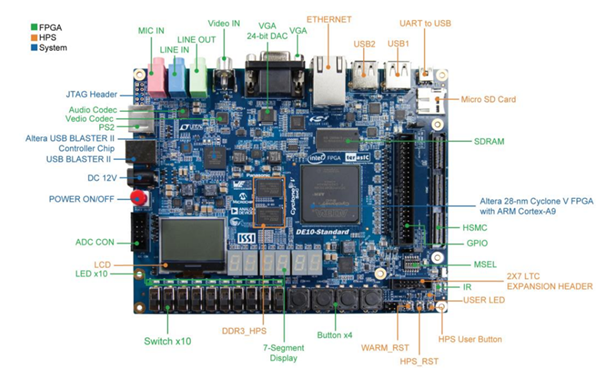
\includegraphics[width=.7\linewidth]{./my-chapters/my-images/theoretical_background/DE_10_board.png}
	\caption{DE10-Standard development board.}
	\label{fig: DE10-Standard development board}
\end{figure}

The DE10-Standard board has many features that allow users to implement a wide range of designed circuits, from simple circuits to various multimedia projects.

The following hardware is provided on the board:

\begin{itemize}[label=-]
	\item \textbf{FPGA}
		\begin{itemize}[label=+]
			\item \text{Altera Cyclone\textsuperscript{\textregistered}} V SE 5CSXFC6D6F31C6N device
			\item Altera serial configuration device – EPCS128 
			\item USB-Blaster II onboard for programming; JTAG Mode
			\item 64MB SDRAM (16-bit data bus)
			\item 4 push-buttons
			\item 10 slide switches
			\item 10 red user LEDs
			\item Six 7-segment displays
			\item Four 50MHz clock sources from the clock generator
			\item 24-bit CD-quality audio CODEC with line-in, line-out, and microphone-in jacks
			\item VGA DAC (8-bit high-speed triple DACs) with VGA-out connector
			\item TV decoder (NTSC/PAL/SECAM) and TV-in connector
			\item PS/2 mouse/keyboard connector
			\item IR receiver and IR emitter
			\item One HSMC with Configurable I/O standard 1.5/1.8/2.5/3.3
			\item One 40-pin expansion header with diode protection
			\item A/D converter, 4-pin SPI interface with FPGA
		\end{itemize}
	\item \textbf{HPS (Hard Processor System)}
		\begin{itemize}[label=+]
			\item 800MHz Dual-core ARM Cortex-A9 MPCore processor
			\item 1GB DDR3 SDRAM (32-bit data bus)
			\item 1 Gigabit Ethernet PHY with RJ45 connector
			\item 2-port USB Host, normal Type-A USB connector
			\item Micro SD card socket
			\item Accelerometer (I2C interface + interrupt)
			\item UART to USB, USB Mini-B connector
			\item Warm reset button and cold reset button
			\item One user button and one user LED
			\item LTC 2x7 expansion header
			\item 128x64 dots LCD Module with Backlight
		\end{itemize}
\end{itemize}

\subsubsection{Block Diagram of the DE10-Standard Board}

\begin{figure}[H]
	\centering
	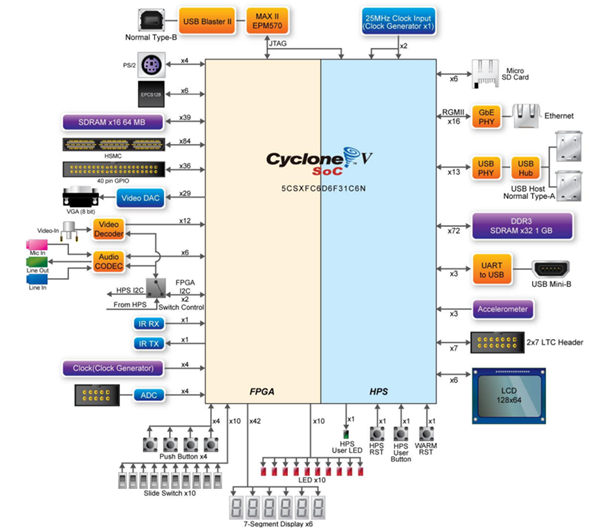
\includegraphics[width=0.7\linewidth]{./my-chapters/my-images/theoretical_background/DE_10_block_diagram.png}
	\caption{Block diagram of DE10-Standard.}
	\label{fig: DE10_blockdiagram}
\end{figure}

All the connections are established through the Cyclone V SoC FPGA device to provide maximum flexibility for users. Detailed information about \ref{fig: DE10_blockdiagram}:

\begin{itemize}[label=-]
	\item \textbf{FPGA Device}
	\begin{itemize}[label=+]
		\item Cyclone V SoC 5CSXFC6D6F31C6N Device
		\item Dual-core ARM Cortex-A9 (HPS)
		\item 110K programmable logic elements
		\item 5,140 Kbits embedded memory
		\item 6 fractional PLLs
		\item 2 hard memory controllers
		\item 3.125G transceivers
	\end{itemize}
	
	\item \textbf{Configuration and Debug}
	\begin{itemize}[label=+]
		\item Quad serial configuration device – EPCS128 on FPGA
		\item Onboard USB-Blaster II (normal type B USB connector)
	\end{itemize}
	
	\item \textbf{Memory Device}
	\begin{itemize}[label=+]
		\item 64MB (32Mx16) SDRAM on FPGA
		\item 1GB (2x256Mx16) DDR3 SDRAM on HPS
		\item Micro SD card socket on HPS
	\end{itemize}
	
	\item \textbf{Communication}
	\begin{itemize}[label=+]
		\item Two port USB 2.0 Host (ULPI interface with USB type A connector)
		\item UART to USB (USB Mini-B connector)
		\item 10/100/1000 Ethernet
		\item PS/2 mouse/keyboard
		\item IR emitter/receiver
		\item I2C multiplexer
	\end{itemize}
	
	\item \textbf{Connectors}
	\begin{itemize}[label=+]
		\item One HSMC (8-channel Transceivers, Configurable I/O standards 1.5/1.8/2.5/3.3V)
		\item One 40-pin expansion headers
		\item One 10-pin ADC input header
		\item One LTC connector (SPI Master, I2C, and GPIO interface)
	\end{itemize}
	
	\item \textbf{Display}
	\begin{itemize}[label=+]
		\item 24-bit VGA DAC
		\item 128x64 dots LCD Module with Backlight
	\end{itemize}
	
	\item \textbf{Audio}
	\begin{itemize}[label=+]
		\item 24-bit CODEC, Line-in, Line-out, and microphone-in jacks
	\end{itemize}
	
	\item \textbf{Video Input}
	\begin{itemize}[label=+]
		\item TV decoder (NTSC/PAL/SECAM) and TV-in connector
	\end{itemize}
	
	\item \textbf{ADC}
	\begin{itemize}[label=+]
		\item Interface: SPI
		\item Fast throughput rate: 500 KSPS
		\item Channel number: 8
		\item Resolution: 12-bit
		\item Analog input range: 0 $\sim$ 4.096 V
	\end{itemize}
	
	\item \textbf{Switches, Buttons, and Indicators}
	\begin{itemize}[label=+]
		\item 5 user Keys (FPGA x4, HPS x1)
		\item 10 user switches (FPGA x10)
		\item 11 user LEDs (FPGA x10, HPS x1)
		\item 2 HPS reset buttons (HPS\_RESET\_n and HPS\_WARM\_RST\_n)
		\item Six 7-segment displays
	\end{itemize}
	
	\item \textbf{Sensors}
	\begin{itemize}[label=+]
		\item G-Sensor on HPS
	\end{itemize}
	
	\item \textbf{Power}
	\begin{itemize}[label=+]
		\item 12V DC input
	\end{itemize}
\end{itemize}


\subsection{Direct Digital Synthesis (DDS)}

DDS is a method of generating different Analog waveforms using digital techniques. It operates by saving the points of a waveform in its digital form. Then it reconstructs the waveform by recalling these digital data. It is a technique which uses digital data and analog signal processing blocks to generate signal waveforms that are repetitive in nature. Many years ago, these digital synthesizers were limited by the clock frequency, which would hinder the speed of operation of the digital logic. Now, with increasing frequency, the limits of the DDS are also increasing.

The technique uses digital data processing to generate a frequency- and phase-tunable output related to a fixed frequency reference, or clock source. In a DDS architecture, the reference or system clock frequency is divided down by the scaling factor, set by a programmable binary tuning word. The tuning word is typically 24-48 bits long which enables a DDS implementation to provide superior output frequency tuning resolution.
Today’s cost-competitive, high-performance, functionally-integrated, and small package-sized DDS products are fast becoming an alternative to traditional frequency-agile analog synthesizer solutions. The integration of a high-speed, high-performance, D/A converter and DDS architecture onto a single chip (forming what is commonly known as a Complete-DDS solution) enabled this technology to target a wider range of applications and provide, in many cases, an attractive alternative to analog-based PLL synthesizers. For many applications, the DDS solution holds some distinct advantages over the equivalent agile analog frequency synthesizer employing PLL circuitry.

Simply stated, a direct digital frequency synthesizer translates a train of clock pulses into an analog waveform, typically a sine, triangular, or square wave. As Figure 1 shows, its essential parts are: a \textit{phase accumulator}, which produces a number corresponding to a phase angle of the output waveform, a \textit{phase-to-digital converter(LUT)}, which generates the instantaneous digital fraction of the output amplitude occurring at a particular phase angle, and a \textit{digital-to-analog converter (DAC)}, which converts that digital value to a sampled analog data point.

\begin{figure}[H]
	\centering
	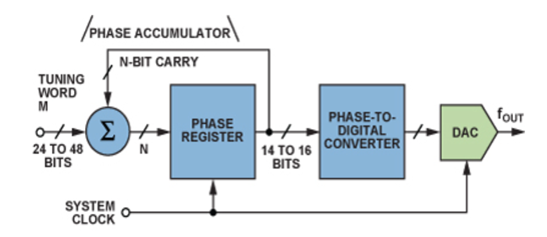
\includegraphics[width=.8\linewidth]{./my-chapters/my-images/theoretical_background/DDS_blockdiagram.png}
	\caption{Functional block diatram for DDS system.}
	\label{fig: DDS_blockdiagram}
\end{figure}

On each clock cycle, the phase accumulator adds a fixed value known as the \textit{frequency tuning word (fcw)}. The result is a digital ramp representing phase over time, which is used to address the LUT. The LUT stores samples of the desired waveform (typically a sine wave), and the output is then converted to analog by the DAC and smoothed by the LPF.

For sine-wave outputs, the phase-to-digital converter is usually a sine lookup table in figure 

\begin{figure}[H]
	\centering
	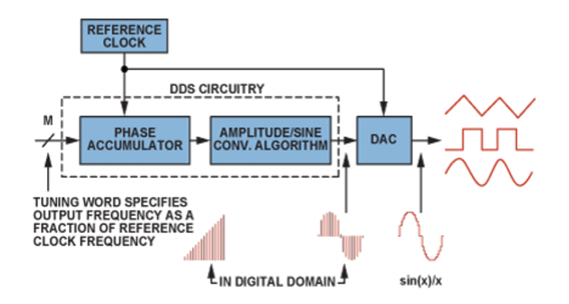
\includegraphics[width=.8\linewidth]{./my-chapters/my-images/theoretical_background/DDS_architecture.png}
	\caption{Typical DDS architecture and signal path with DAC.}
	\label{fig: DDS_architecture}
\end{figure}

\subsection{Phase accumulator and how to generate waveform}

The Phase Accumulator is an $n$-bit register that operates with modulo $2^n$ arithmetic. 
At every clock cycle, it adds a fixed value $M$, called the \textbf{Frequency Control Word (FCW)} or tuning word, to its current phase value.

\begin{itemize}[label=-]
	\item The \textbf{FCW} determines the phase step size.
	\item A larger FCW increases the phase more quickly $\Rightarrow$ higher output frequency.
	\item A smaller FCW increases the phase more slowly $\Rightarrow$ lower output frequency.
\end{itemize}

\noindent
\textbf{Operating principle:}  
On each rising edge of the system clock, the accumulator updates its value by adding the FCW. 
This process creates a steadily increasing phase ramp that cycles from $0$ to $2^n-1$. 
When the maximum value is reached, the accumulator \textbf{overflows} and wraps around to $0$, similar to a clock hand completing a full revolution. 
This mechanism is often called a \textit{digital phase wheel} as show in Figure \ref{fig: banh xe pha}.

\begin{figure}[H]
	\centering
	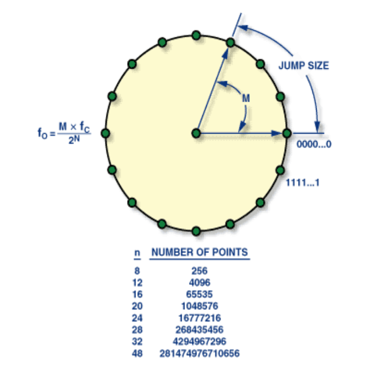
\includegraphics[width=.6\linewidth]{./my-chapters/my-images/Gen_wave/hinh1.png}
	\caption{Digital phase wheel.}
	\label{fig: banh xe pha}
\end{figure}

\[
f_{out} = \frac{M}{2^n} \cdot f_{clk}
\]

where:
\begin{itemize}[label=+]
	\item $f_{out}$ : output frequency
	\item $f_{clk}$ : system clock frequency
	\item $M$ : Frequency Control Word (FCW)
	\item $n$ : number of bits in the phase accumulator
\end{itemize}

\subsection{Concept of Waveform Generation}

\subsubsection{Sine Wave}

Implementation idea: The total has $1024$ samples, which means storing the entire $0^{\circ} \rightarrow 360^{\circ}$ range for one full sine wave cycle. However, this would require four times the ROM size $\rightarrow$ instead, it is sufficient to store only $\dfrac{1}{4}$ of the cycle, that is $0^{\circ} \rightarrow 90^{\circ}$.

First, the MSB bit is used to distinguish between the positive sine region ($0^{\circ} \rightarrow 180^{\circ}$, the first two quadrants) and the negative sine region ($180^{\circ} \rightarrow 360^{\circ}$, the last two quadrants). Next, within each region, the bit [MSB-1] is used as a symmetry marker to indicate when the address should be mirrored, thereby producing a complete half sine wave.

For the first positive half cycle, the phase step is selected depending on the desired output frequency. The phase accumulator will accumulate and gradually increase the address in the first quadrant according to the stored $\dfrac{1}{4}$ samples when bit [MSB-1] = 0. If bit [MSB-1] = 1, then a mirror operation is performed by taking the Maximum – address of the first quadrant or simply applying the NOT operation to the address. This produces the second quadrant and completes the first positive half cycle of the sine wave.

For the negative half cycle, a two’s complement operation is required to switch from positive to negative values when MSB = 1. Then, mirroring is applied to obtain the third quadrant. Finally, the last quadrant is mirrored again from the third quadrant.

In summary, the MSB determines the positive or negative region, while bit [MSB-1] determines whether mirroring is applied or not.

\subsubsection{ECG Waveform}

Since the ECG waveform is complex, the group uses a HEX file as the LUT with 1024 samples. Similarly, the phase accumulator accumulates phase and increases the address, with each address containing one amplitude value of the ECG signal. As a result, the ROM sequentially outputs each ECG sample. By combining these samples over time, a complete ECG waveform is formed.

\subsubsection{Square Wave}

For the square wave, the implementation is simpler and does not require a LUT. Specifically:

The phase accumulator acts as a “time ruler” for one waveform cycle. A square wave has two levels: HIGH (24'h0FFF00) and LOW (24'h0). The waveform is determined by comparing the accumulated phase with predefined thresholds.

The duty cycle values are selected as desired. From this, the threshold values are determined to switch between HIGH and LOW. For example, with a duty cycle of 90\% of 1024 samples, it requires counting $10’d102$ samples to create the LOW level first, and this count is chosen as the threshold. Once the threshold is exceeded, the signal switches to HIGH. The same approach is used for other duty cycle values.

For some special duty cycles such as 50\%, the symmetry of the MSB can be exploited. After counting half a cycle with MSB = 0, the state changes at MSB = 1. For 75\% or 25\% duty cycles, an OR operation between the two MSB bits can be used.

\subsubsection{Sawtooth Wave}

The sawtooth waveform is generated by accumulating phase, similar to other waveforms. By exploiting the wrap-around phenomenon, the phase increases linearly as a ramp and resets immediately to 0 when overflow occurs.

\subsubsection{Triangle Wave}

The triangle waveform is derived from the sawtooth waveform with two linear ramps: one increasing in the first half and one decreasing in the second half. This is implemented by accumulating phase to form a linear ramp (sawtooth), then exploiting symmetry with the MSB to invert the ramp in the second half, or by taking Maximum – accumulated value from the first ramp.

\subsection{Configuration for the WM8731 Audio Codec}
\subsubsection{Audio Codec WM8731 Overview}

\begin{figure}[H]
	\centering
	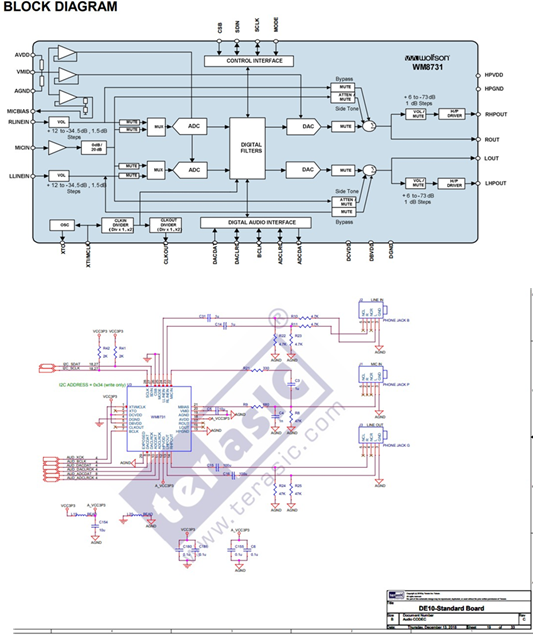
\includegraphics[width=0.7\linewidth]{./my-chapters/my-images/theoretical_background/WM8731_blockdiagram.png}
	\caption{Block Diagram of the Integrated ADC/DAC Audio Codec in the WM8731.}
\end{figure}

\begin{enumerate}[label=\alph*)]
	
	\item \textbf{Role:} The WM8731 is an integrated audio ADC/DAC that supports stereo audio signal processing.  
	
	\item \textbf{Application:} It is used for audio capture/playback via the I$^2$S interface and is configured through I$^2$C/SPI.  
	
	\item \textbf{Supported Modes:} The WM8731 provides multiple operating features:
	\begin{itemize}[label=-]
		\item 24-bit ADC and DAC using sigma-delta architecture with digital decimation/interpolation filters, providing high SNR and noise reduction.  
		\item Control interface via two-wire or three-wire communication (commonly I$^2$C) for full access to configuration registers (volume, mute, de-emphasis, and other modes).  
		\item Digital audio data interface supporting multiple formats (I$^2$S, Left Justified, Right Justified, DSP mode), with data word lengths from 16 to 24 bits, and sampling rates from 8 kHz to 96 kHz.  
		\item Utility functions: integrated headphone driver with efficient output stage, mute function, and flexible power management system with multiple power-down modes for individual blocks.  
	\end{itemize}
	
	\item \textbf{Important Pins:}
	\begin{table}[H]
		\centering
		\caption{Key WM8731 Connections with DE10}
		\label{tab:wm8731_pins}
		\begin{tabular}{|>{\centering\arraybackslash}m{2cm}
				|>{\centering\arraybackslash}m{6cm}
				|>{\centering\arraybackslash}m{8cm}|}
			\hline
			\textbf{WM8731 Pin} & \textbf{Connected to DE10} & \textbf{Function} \\ \hline
			SCLK   & I2C\_SCLK (I$^2$C clock)      & I$^2$C clock \\ \hline
			SDIN   & I2C\_SDAT (I$^2$C data)       & I$^2$C data \\ \hline
			MCLK (XTI) & AUD\_XCK {[3:0]}           & Main codec clock (typically 12 MHz or 18.432 MHz) \\ \hline
			BCLK   & AUD\_BCLK {[3:0]}             & I$^2$S bit clock (e.g., 3.072 MHz = 48 kHz $\times$ 64) \\ \hline
			DACLRC & AUD\_DACLRCK {[3:0]}          & Left/Right clock for DAC \\ \hline
			DACDAT & AUD\_DACDAT {[3:0]}           & I$^2$S data output, audio data from FPGA $\to$ WM8731 \\ \hline
		\end{tabular}
	\end{table}
	Pins \texttt{SCLK} and \texttt{SDIN} require pull-up resistors (2.2k$\Omega$–10k$\Omega$) to ensure reliable I$^2$C operation.  
	The master clock (\texttt{MCLK}) must be generated by the DE10 PLL with precise frequency (e.g., 12.288 MHz for a 48 kHz sampling rate).  
	
	\item \textbf{I$^2$C Addressing:}  
	In the I$^2$C protocol, each device is assigned a 7-bit (or sometimes 10-bit) address. For the DE10 system, the WM8731 codec is configured as a slave device with the I$^2$C address \texttt{0x34} (write-only mode).  
	
	Since WM8731 only supports configuration via write operations, the effective 7-bit slave address is:  
	\[
	0x34 \ (\text{hex}) = 0110100 \ (\text{binary})
	\]  
	
	The 8-bit I$^2$C frame address is then:  
	\[
	0x68 \ (\text{hex}) = 01101000 \ (\text{binary})
	\]  
	where the 7-bit device address is followed by a single R/W bit (set to 0 for write).
	
\end{enumerate}


\subsubsection{Register Configuration for WM8731}

The WM8731 codec is configured to operate according to the requirements of the Lab. 
These configuration registers are transmitted via the $I^{2}C$ protocol.

% ========================
% Longtable format
% ========================
\begin{longtable}{|>{\centering\arraybackslash}m{1.2cm}
		|>{\centering\arraybackslash}m{1.5cm}
		|>{\centering\arraybackslash}m{1.5cm}
		|>{\raggedright\arraybackslash}m{3cm}
		|>{\raggedright\arraybackslash}m{7cm}|}
	\caption{Register configuration for WM8731} \label{tab:wm8731} \\ 
	\hline
	\textbf{Index} & \textbf{Address} & \textbf{Data} & \textbf{Register} & \textbf{Function} \\
	\hline
	\endfirsthead
	
	% ========================
	% Header for the following pages
	% ========================
	\multicolumn{5}{c}%
	{{\bfseries Table \thetable\ Register configuration for WM8731}} \\
	\hline
	\textbf{Index} & \textbf{Address} & \textbf{Data} & \textbf{Register} & \textbf{Function} \\
	\endhead
	
	% ========================
	% Footer for intermediate pages
	% ========================
	\multicolumn{5}{r}{{Next page...}} \\
	\endfoot
	
	% ========================
	% Footer for the last page
	% ========================
	\endlastfoot
	
	% ========================
	% Table content
	% ========================
	0  & 0x0F & 0x00 & Reset Register               & Reset the entire codec to its default state \\ \hline
	1  & 0x06 & 0x10 & Power Down Control           & Disable MIC input, enable LINEOUT, LINEIN, ADC, DAC \\ \hline
	2  & 0x02 & 0x79 & Left Headphone Out           & Left headphone volume: 0 dB, Zero-Cross detect enabled \\ \hline
	3  & 0x03 & 0x79 & Right Headphone Out          & Right headphone volume: 0 dB, Zero-Cross detect enabled \\ \hline
	4  & 0x00 & 0x17 & Left Line In                 & Left line-in volume: 0 dB, not muted \\ \hline
	5  & 0x01 & 0x17 & Right Line In                & Right line-in volume: 0 dB, not muted \\ \hline
	6  & 0x04 & 0x10 & Analog Audio Path Control    & Select LINEIN $\to$ ADC, disable MIC, disable bypass, enable DAC \\ \hline
	7  & 0x05 & 0x00 & Digital Audio Path Control   & Disable high-pass filter, disable de-emphasis, disable DAC soft-mute \\ \hline
	8  & 0x07 & 0x0A & Digital Audio Interface Format & Select Left-justified mode, 24-bit, MSB first \\ \hline
	9  & 0x08 & 0x01 & Sampling Control             & USB mode, MCLK = 12 MHz, Fs = 48 kHz \\ \hline
	10 & 0x09 & 0x01 & Active Control               & Activate codec (ACTIVE = 1) \\ \hline
	11 & 0x06 & 0x02 & Power Down Control           & Keep ADC, DAC, LINEIN, LINEOUT active; only power down Microphone \\ \hline
	
\end{longtable}

\subsubsection{I$^2$C Protocol}

\begin{enumerate}[label=\alph*) ]
	\item \textbf{Overview:}
	
	I$^2$C stands for \textbf{Inter-Integrated Circuit}. It is a bus interface connection protocol incorporated into devices for serial communication. It was originally designed by Philips Semiconductor in 1982. Recently, it has become a widely used protocol for short-distance communication. It is also known as the \textit{\textbf{Two-Wired Interface (TWI)}}.

	I$^2$C uses only two bi-directional open-drain lines for data communication, called \textbf{SDA} and \textbf{SCL}. Both these lines are pulled high.
	\begin{itemize}[label=-]
		\item \textit{Serial Data (SDA):} Transfer of data takes place through this pin.
		\item \textit{Serial Clock (SCL):} It carries the clock signal.
	\end{itemize}
	
	I$^2$C operates in two modes:
	\begin{itemize}[label=-]
		\item Master mode
		\item Slave mode
	\end{itemize}
	
	According to the I$^2$C protocol rules, the data line cannot change when the clock line is high; it can change only when the clock line is low. Since the two lines are \textit{open-drain}, pull-up resistors are required to keep the lines at a high level, as the devices on the I$^2$C bus are active low.
	
	\begin{figure}[H]
		\centering
		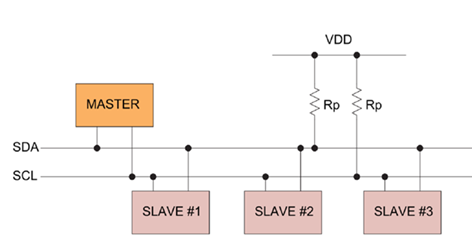
\includegraphics[width=.7\linewidth]{./my-chapters/my-images/theoretical_background/TWI_communication.png}
		\caption{Generalized I$^{2}$C Connection Diagram.}
		\label{fig: TWI protocol connection diagram}
	\end{figure}
	
	\item \textbf{How I$^2$C works:}
	
	With I$^{2}$C, data is transferred to \textbf{messages}. Messages are broken up into \textbf{frames} of data. Each message has an address frame that contains the binary address of the slave, and one or more data frames that contain the data being transmitted. The message also includes start and stop conditions, read/write bits, and ACK/NACK bits between each data frame:

	\begin{figure}[H]
		\centering
		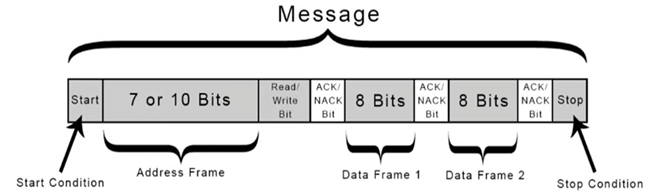
\includegraphics[width=0.7\linewidth]{./my-chapters/my-images/theoretical_background/TWI_Messages are broken up into frames of data.png}
		\caption{Messages are broken up into frames of data.}
		\label{fig: TWI_Messages are broken up into frames of data}
	\end{figure}
	
	\begin{itemize}[label=-]
		\item \textit{Start Condition:} The SDA line switches from a high voltage level to a low voltage level before the SCL line switches from high to low.
		\item \textit{Stop Condition:} The SDA line switches from a low voltage level to a high voltage level after the SCL line switches from low to high.
		
		\begin{figure}[H]
			\centering
			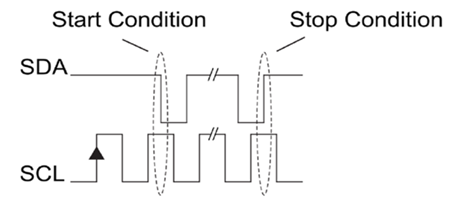
\includegraphics[width=0.7\linewidth]{./my-chapters/my-images/theoretical_background/TWI_start_condition.png}
			\caption{Start Condition And Stop Condition Transitions.}
			\label{fig: TWI_start_condition}
		\end{figure}
		
		\item \textit{Address:} Frame: A 7- or 10-bit sequence unique to each slave that identifies the slave when the master wants to talk to it.
		\item \textit{Read/Write Bit:} A single bit specifying whether the master is sending data to the slave (low voltage level) or requesting data from it (high voltage level).
		\item \textit{ACK/NACK Bit:} Each frame in a message is followed by an acknowledge/no-acknowledge bit. If an address frame or data frame was successfully received, an ACK bit is returned to the sender from the receiving device.
	\end{itemize}
	
	\item \textbf{Addressing}
	
	I$^{2}$C doesn’t have slave select lines like SPI, so it needs another way to let the slave know that data is being sent to it, and not another slave. It does this by addressing. The address frame is always the first frame after the start bit in a new message.  
	
	The master sends the address of the slave it wants to communicate with to every slave connected to it. Each slave then compares the address sent from the master to its own address. If the address matches, it sends a low voltage \textit{ACK} bit back to the master. If the address doesn’t match, the slave does nothing, and the \textit{SDA} line remains high.  
	
	A slave address is sent in 8-bit byte format, MSB first, but the last bit signifies whether the transaction will be read or write to the slave. In effect, the upper 7 bits constitute the slave address, while the 8th bit serves as a \textit{READ/WRITE} command bit. Thus, there is an address space of 128 unique addresses for addressing up to 128 slaves.
	
	\item \textbf{Acknowledge and Not Acknowledge Bits (ACK/NACK)}
	
	As a form of feedback, after every byte transmission the receiving device sends an Acknowledge or Not Acknowledge bit. An Acknowledge bit is generated by the receiver by holding the SDA line low during a HIGH \textit{SCL} period, while a Not Acknowledge bit is generated when the receiver leaves the \textit{SDA} line passively pulled HIGH and does not respond in any way. This fact implies that in response to an address byte, all unmatched SLAVEs send a Not Acknowledge bit by not responding.
	
	An ACK is used to denote that a byte (address or data) was transmitted and received successfully and that the transmission can continue to the next byte transfer, a stop condition or a repeated start. A NACK is generally used by the receiver to indicate whether an error occurred somewhere in the data transmission. This is used to signal to the transmitting device to terminate the transmission immediately or to make another attempt by sending a repeated start.
	
	\item \textbf{WM8731 I$^{2}$C Data Transmission Steps}
	
		\begin{enumerate}[label=Step \arabic*., leftmargin=2cm]
			\item The master sends the start condition to every connected slave by switching the \textit{SDA} line from a high voltage level to a low voltage level before switching the \textit{SCL} line from high to low.
			\item The master sends each slave the 7-bit address (for the WM8731, the 7-bit I$^{2}$C slave address is typically \texttt{0x1A}) of the slave it wants to communicate with, along with the read/write bit.
			
			The WM8731 supports a 2-wire MPU serial interface. The device operates as a slave device only. The WM8731 has one of two slave addresses that are selected by setting the state of pin 10, (CSB).
			
				 \begin{table}[h] % or [t], [b], [!ht], etc.
					 \centering
					 \vspace{0.5em} % khoảng cách sau caption
					 \begin{tabular}{|>{\centering\arraybackslash}m{5cm}
							                 |>{\centering\arraybackslash}m{5cm}|}
						\hline
						CBS State 				  & Address \\ 
						(Default = LOW)			  & 		\\ \hline
						0 						  & 0011010 \\ \hline
						1 						  & 0011011 \\ \hline
					\end{tabular}
					\caption{2-Wire MPU Interface Address Selection (Select Slave address to communicate).}
				\end{table}
			
			\item Each slave compares the address sent from the master to its own address. If the address matches, the slave returns an ACK bit by pulling the \textit{SDA} line low for one bit. If the address from the master does not match the slave’s own address, the slave leaves the \textit{SDA} line high.
			\item The master sends or receives the data frame.
			\item After each data frame has been transferred, the receiving device returns another ACK bit to the sender to acknowledge successful receipt of the frame.
			\item After successfully receiving the ACK (confirming that the SLAVE is ready to communicate), SDA will continue sending the configuration register DATA, which consists of the 7-bit register address (DATA $B_{15} - B_{9}$) and the 9-bit configuration value for that register (DATA $B_{8} - B_{0}$), for a total of 16 bits divided into 2 frames.
			
			In the first transmission, the frame containing the register address is sent after the ACK has been received. Since \textit{SDA} sends data in 8-bit frames, the register address frame must take the MSB from the 9-bit register configuration value as the LSB of the address frame and send it first (DATA $B_{15} - B_{8}$).
			
			\item When the data transmission is completed, the process continues by waiting to check whether the ACK bit is returned. If successful, proceed to send the remaining frame, which contains the 8-bit configuration data (DATA $B_{7} - B_{0}$).
			
			\item After transmission, wait for the ACK bit response to verify whether the DATA has been successfully sent.
			\item After confirming that the ACK has been successfully received, proceed to the stop process. To stop the data transmission, the master sends a stop condition to the slave by switching SCL high before switching \textit{SDA} high. When the STOP condition is successfully met, it means the configuration data for one register has been fully transmitted. To perform the same operation for other registers, simply repeat all the steps from the beginning up to the STOP condition.
			
			\begin{figure}[H]
				\centering
				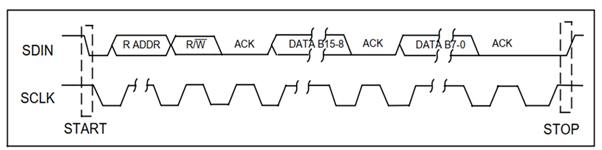
\includegraphics[width=0.7\linewidth]{./my-chapters/my-images/theoretical_background/TWI_protocol.png}
				\caption{2-Wire Serial Interface of WM8731.}
			\end{figure}
		\end{enumerate}
\end{enumerate}

The I$^{2}$C communication protocol is a simple and effective way for devices to communicate with each other. It allows multiple devices to connect using just two wires, making it easy to add new components to a system. I$^{2}$C is popular in various applications because it supports multiple devices, is relatively easy to implement, and requires less wiring compared to other protocols. Overall, I2C is a reliable choice for connecting sensors, displays, and other peripherals in electronic projects.

\subsubsection{$I^{2}S$ Communication Protocol}

The protocol which is used to transmit digital audio data from one device to another is known as I$^{2}$S or Inter-IC Sound protocol. This protocol transmits PCM (pulse-code modulated) audio data from one IC to another within an electronic device. I$^{2}$S plays a key role in transmitting audio files which are pre-recorded from an MCU to a DAC or amplifier. This protocol can also be utilized to digitize audio using a microphone. There is no compression within I$^{2}$S protocols, so you cannot play OGG or MP3 or other audio formats that condense the audio, however, you can play WAV files.

In the WM8731 datasheet, it is specified that I$^{2}$S mode operates as follows:

\textbf{\textit{I$^{2}$S mode is where the MSB (most-significant bit) is available on the 2nd rising edge of BCLK (Bit Clock) following an LRCLK/DACLRC (Left/Right Clock) transition }} - meaning the MSB is delayed by one BCLK compared to the left-justified format. This is the standard method to synchronize left/right channel data with the LRCLK signal, as illustrated in figure \ref{fig: I2S mode} below.

\begin{figure}[H]
	\centering
	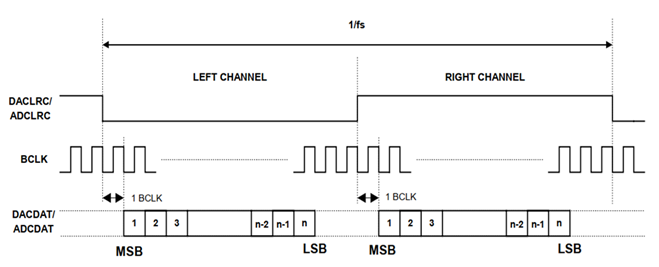
\includegraphics[width=.8\linewidth]{./my-chapters/my-images/theoretical_background/I2S_mode.png}
	\caption{I$^{2}$S mode.}
	\label{fig: I2S mode}
\end{figure}

\textit{LRCLK} must always transition on the falling edge of \textit{BCLK}, as stated in the datasheet. This requirement must be met when interfacing devices in both master and slave modes. Each data bit is changed/shifted on the high-to-low transition of \textit{BCLK} and sampled on the low-to-high transition of \textit{BCLK}.

According to the provided I$^{2}$C register configuration, the WM8731 is set to:

\begin{itemize}[label=-]
	\item\textbf{ Slave Mode:} When WM8731 operates in Slave mode, both BCLK and DACLRC are inputs, as shown in the figure \ref{fig: I2S slave mode}.
	
	\begin{figure}[H]
		\centering
		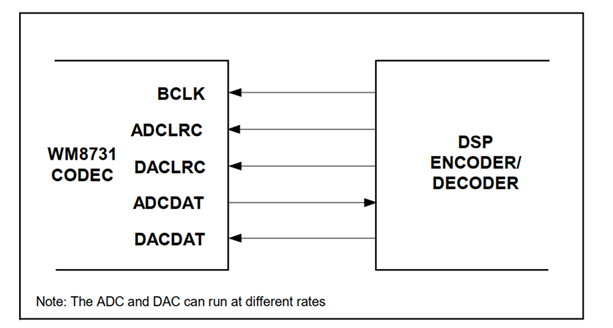
\includegraphics[width=.8\linewidth]{./my-chapters/my-images/theoretical_background/I2S_slave_mode.png}
		\caption{I$^{2}$S slave mode.}
		\label{fig: I2S slave mode}
	\end{figure}
\end{itemize}
\section{Hardware design and Implementation}

\subsection{Module Waveform Generator}

\subsubsection{Module Sine Waveform}
\begin{figure}[H]
	\centering
	\fbox{%
		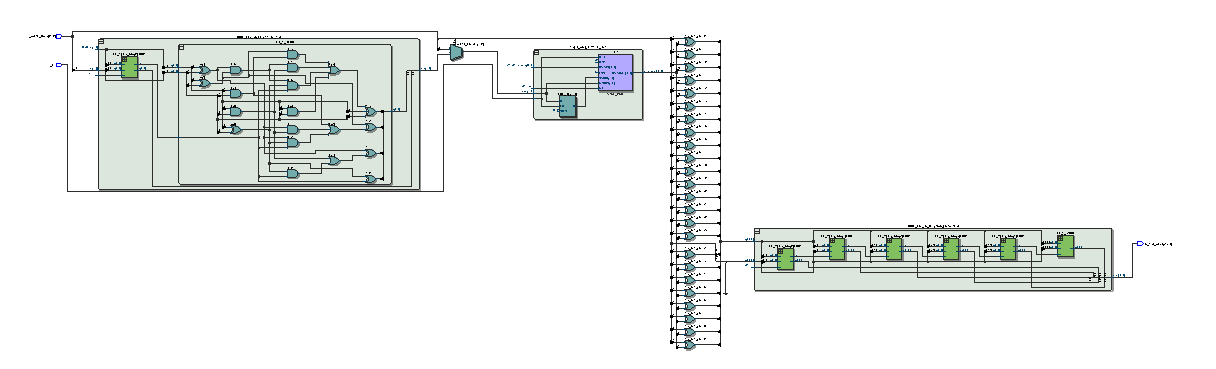
\includegraphics[width=\linewidth]{./my-chapters/my-diagrams/wave_sin.pdf}%
	}
	\caption{Block diagram for Module Sin\_Wave.}
\end{figure}

\subsubsection{Module Square Waveform}
\begin{figure}[H]
	\centering
	\fbox{%
		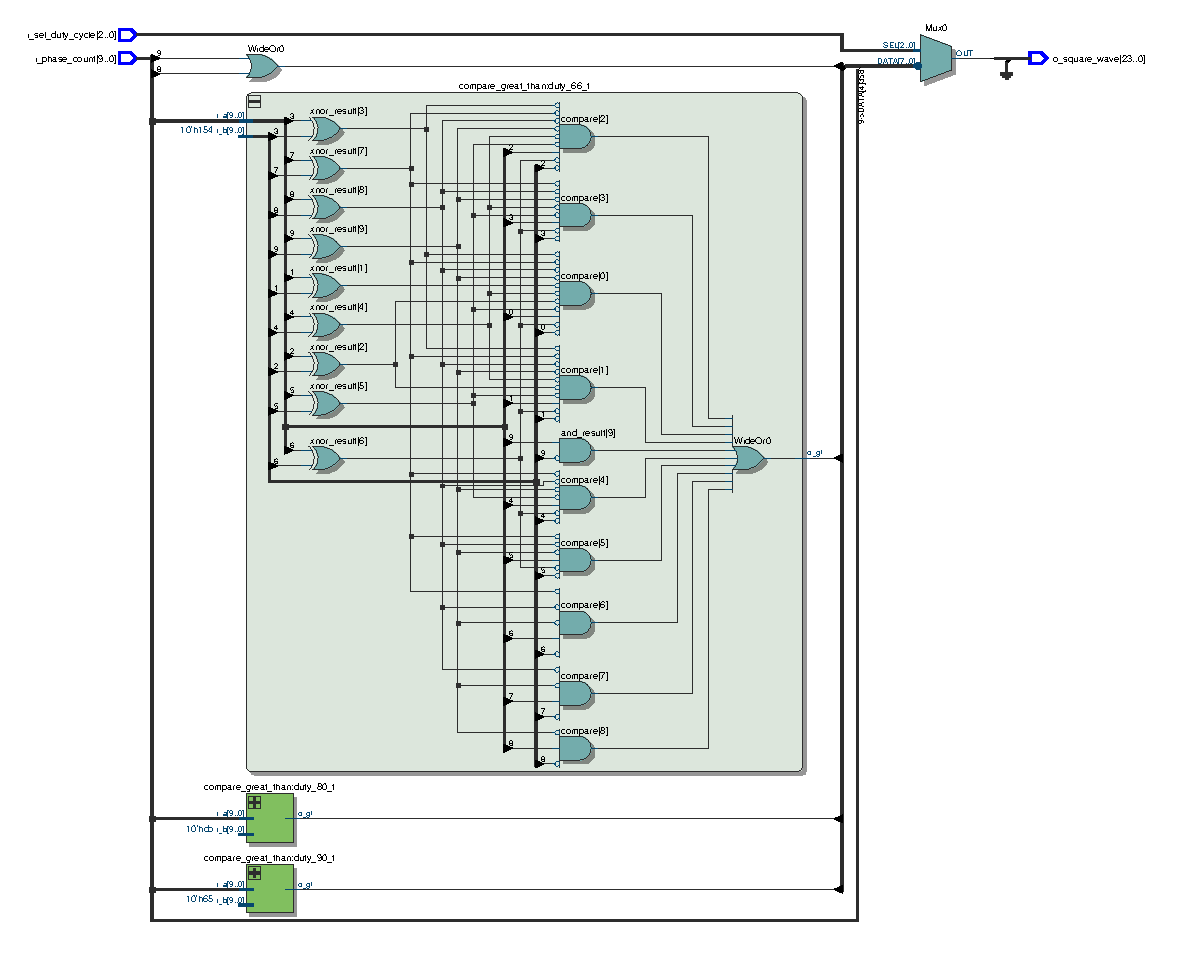
\includegraphics[width=\linewidth]{./my-chapters/my-diagrams/wave_square.pdf}%
	}
	\caption{Block diagram for Module Square\_wave.}
\end{figure}

\subsubsection{Module Triangle Waveform}
\begin{figure}[H]
	\centering
	\fbox{%
		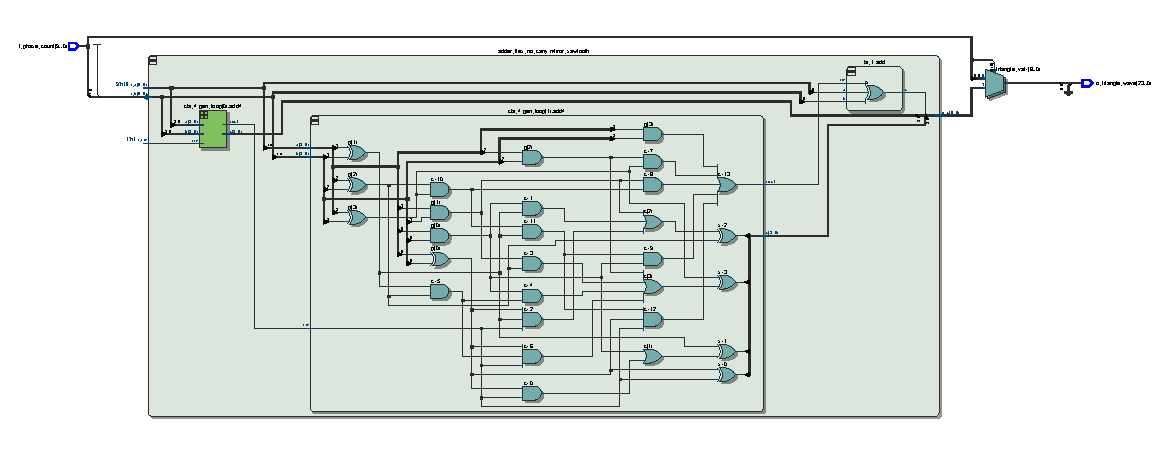
\includegraphics[width=\linewidth]{./my-chapters/my-diagrams/wave_triangle.pdf}%
	}
	\caption{Block diagram for Module Triangle\_wave.}
\end{figure}

\subsubsection{Module Sawtooth Waveform}
\begin{figure}[H]
	\centering
	\fbox{%
		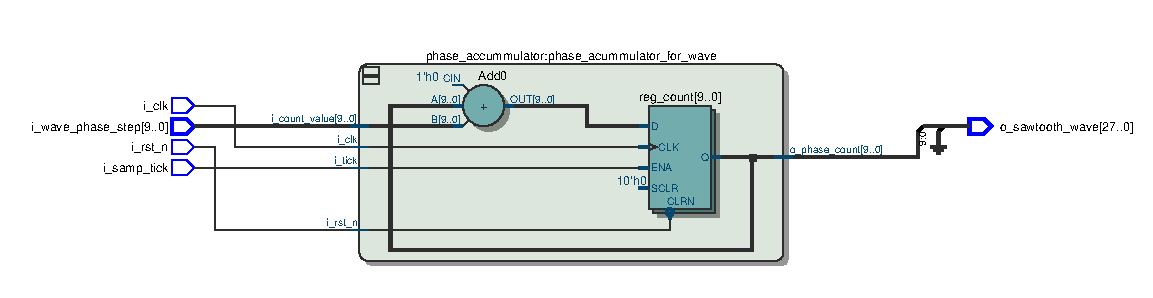
\includegraphics[width=\linewidth]{./my-chapters/my-diagrams/wave_sawtooth.pdf}%
	}
	\caption{Block diagram for Module Sawtooth\_wave.}
\end{figure}

\subsubsection{Module ECG Waveform}
\begin{figure}[H]
	\centering
	\fbox{%
		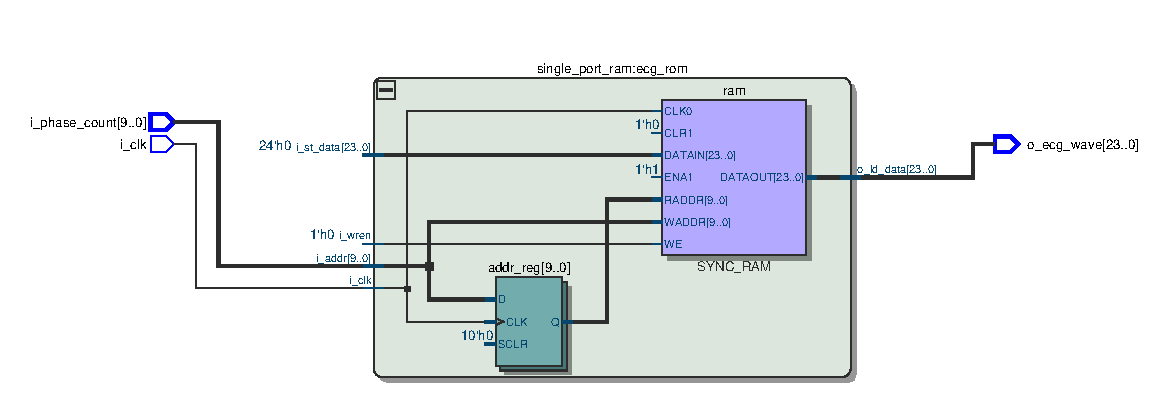
\includegraphics[width=\linewidth]{./my-chapters/my-diagrams/wave_ecg.pdf}%
	}
	\caption{Block diagram for Module ECG\_wave.}
\end{figure}

\subsubsection{Module Waveform Generator}
\begin{figure}[H]
	\centering
	\fbox{%
		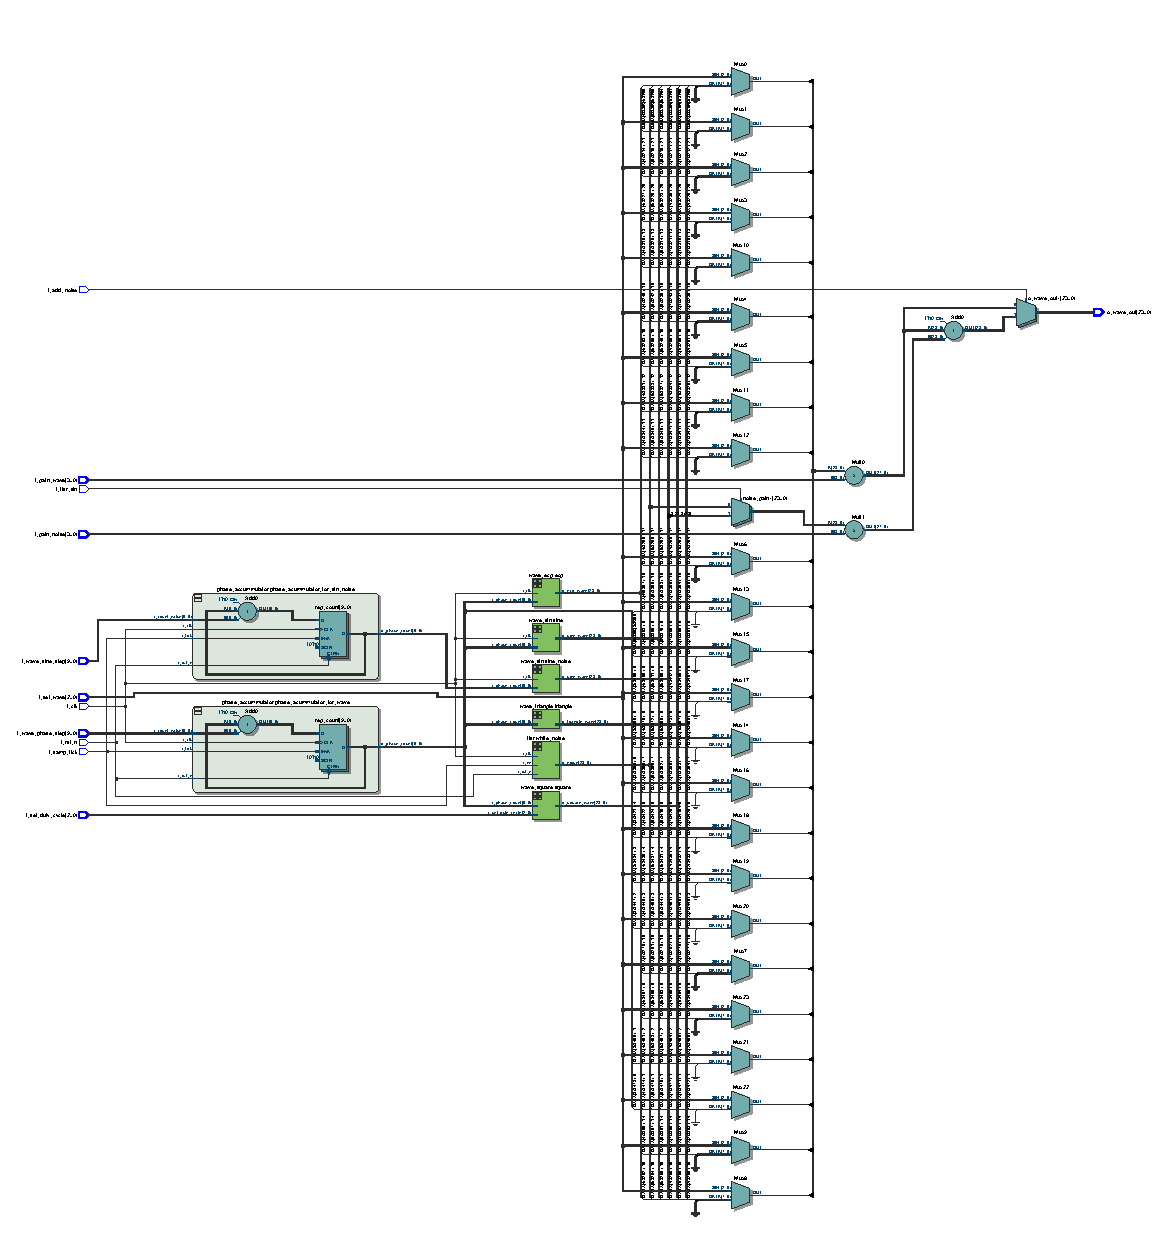
\includegraphics[width=\linewidth]{./my-chapters/my-diagrams/wave_gen.pdf}%
	}
	\caption{Block diagram for Module Waveform Generator.}
\end{figure}

\subsection{Module Control value}

\begin{figure}[H]
	\centering
	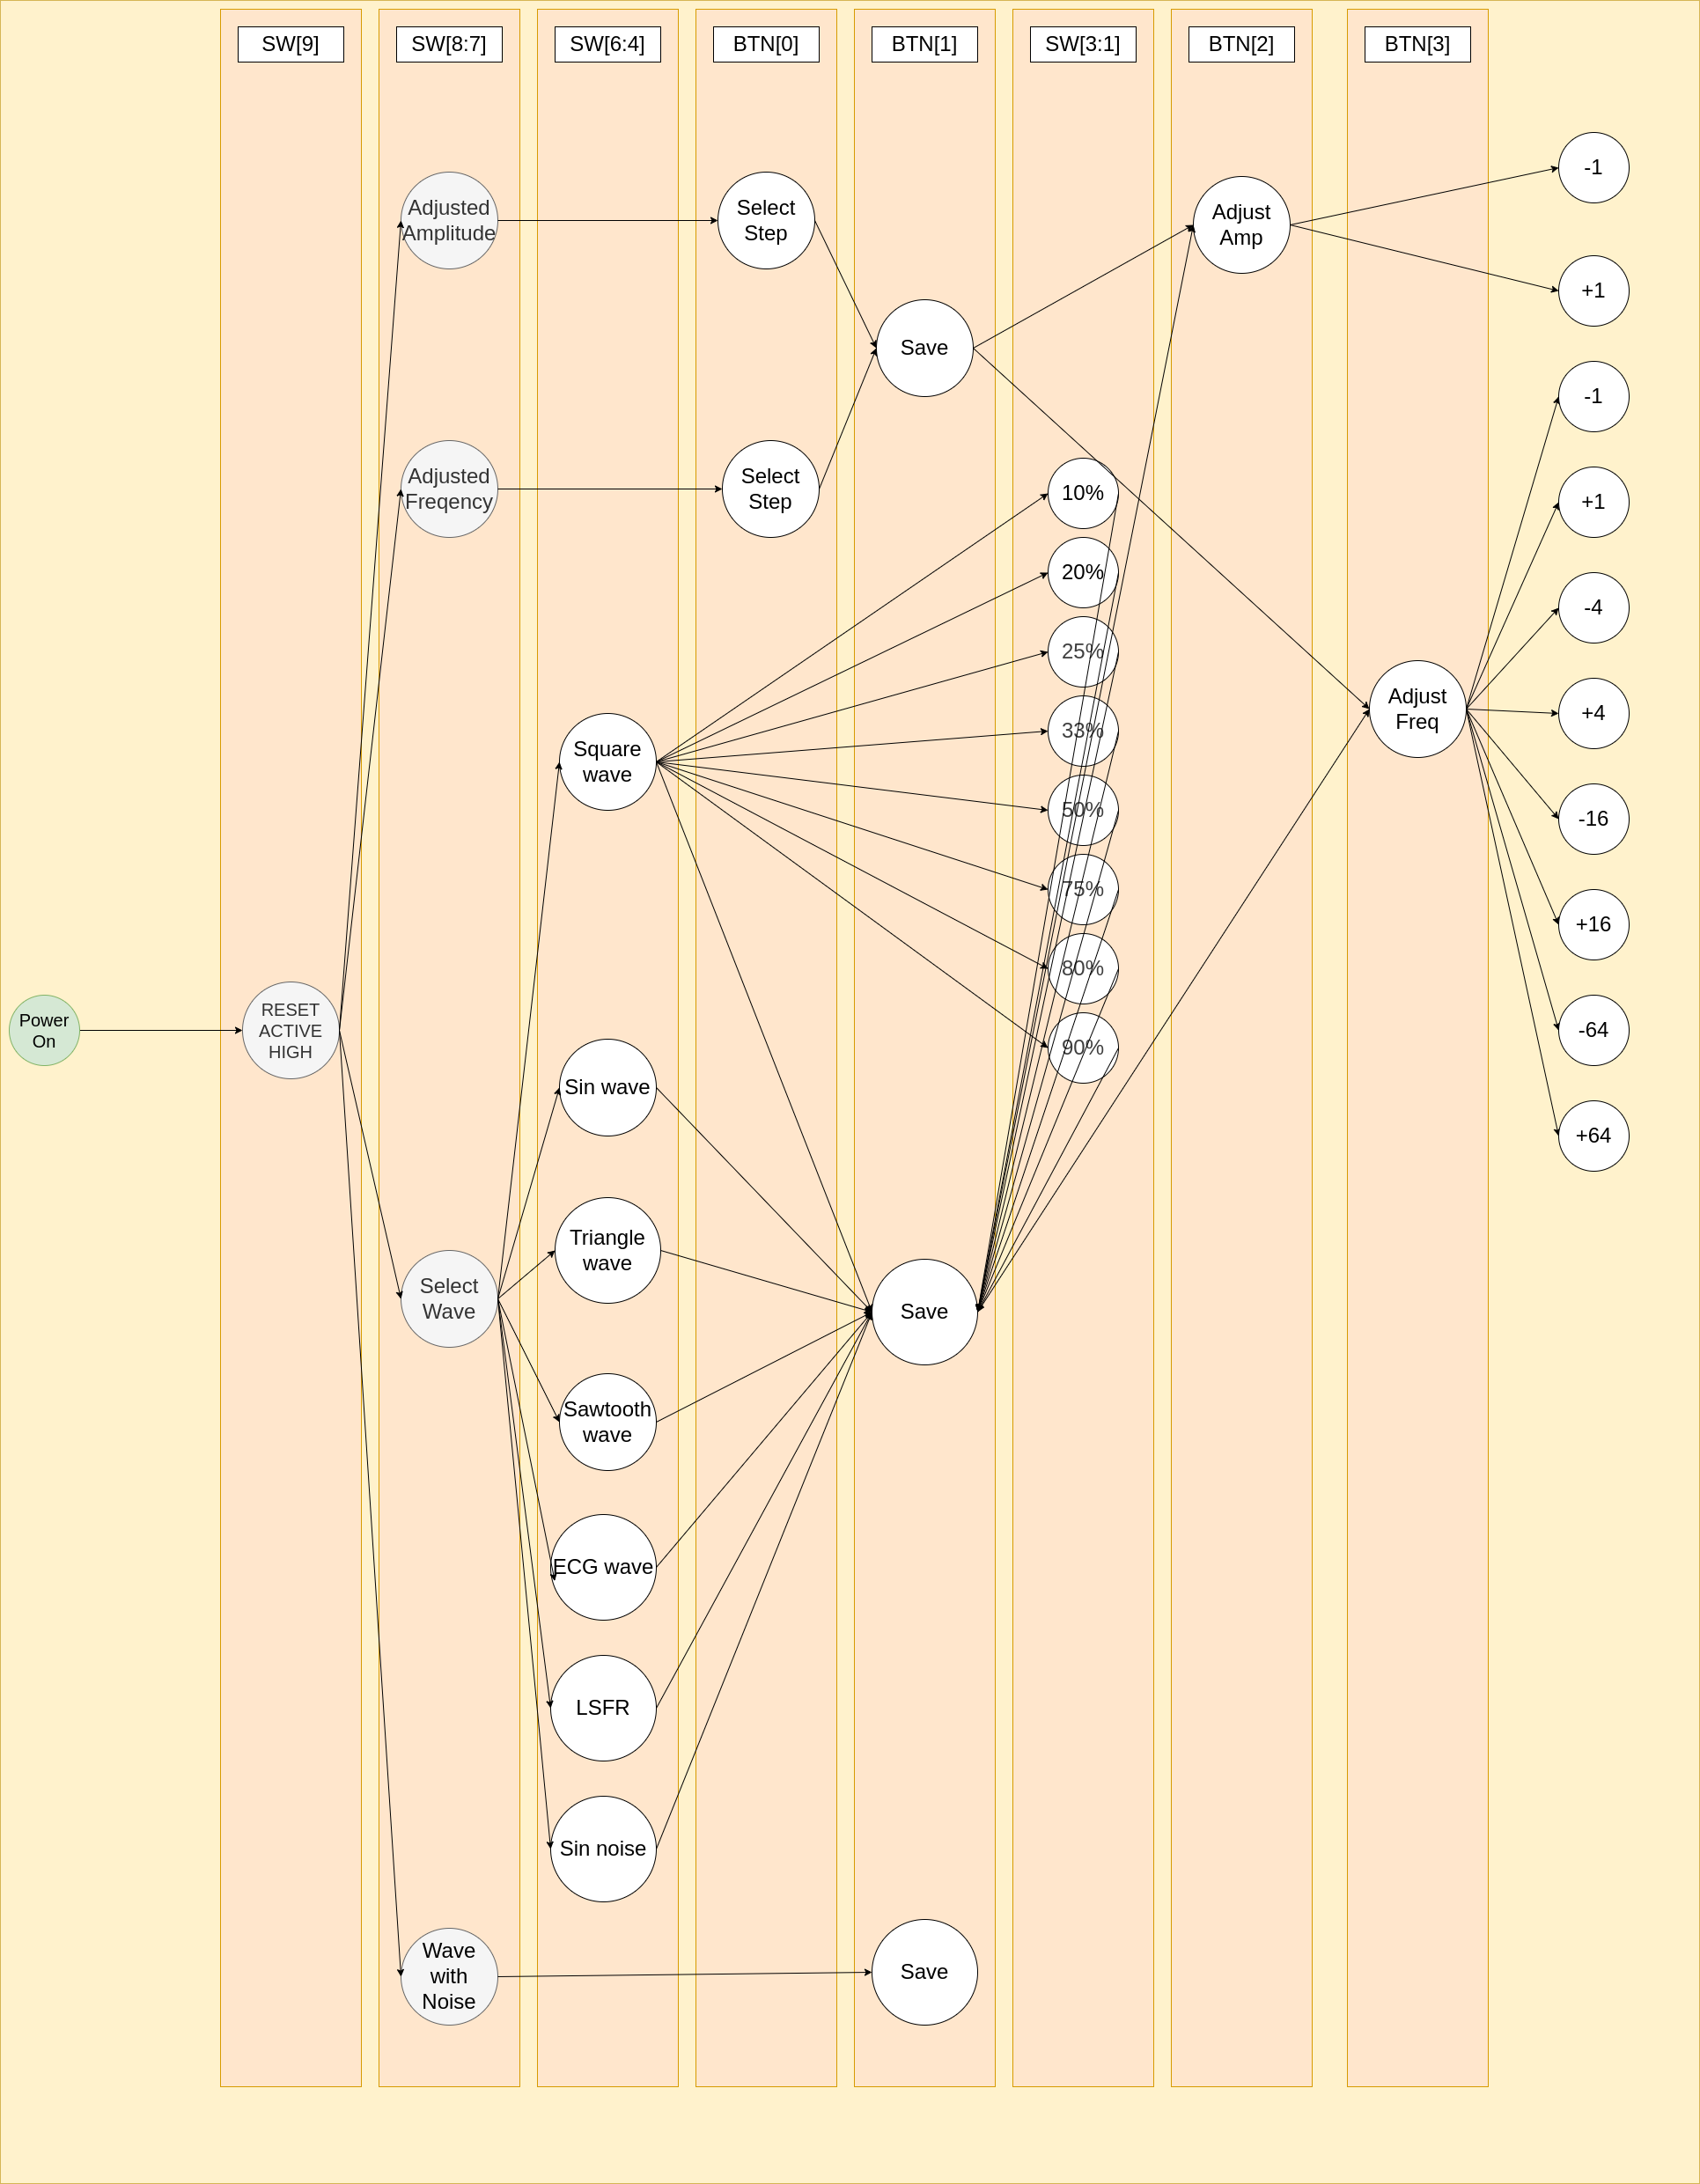
\includegraphics[width=.8\linewidth, height=0.7\textheight]{./../00_spec/spec/UI_task.png}
	\caption{Communication operations between the user and the Control Value Module.}
\end{figure}

\begin{figure}[H]
	\centering
	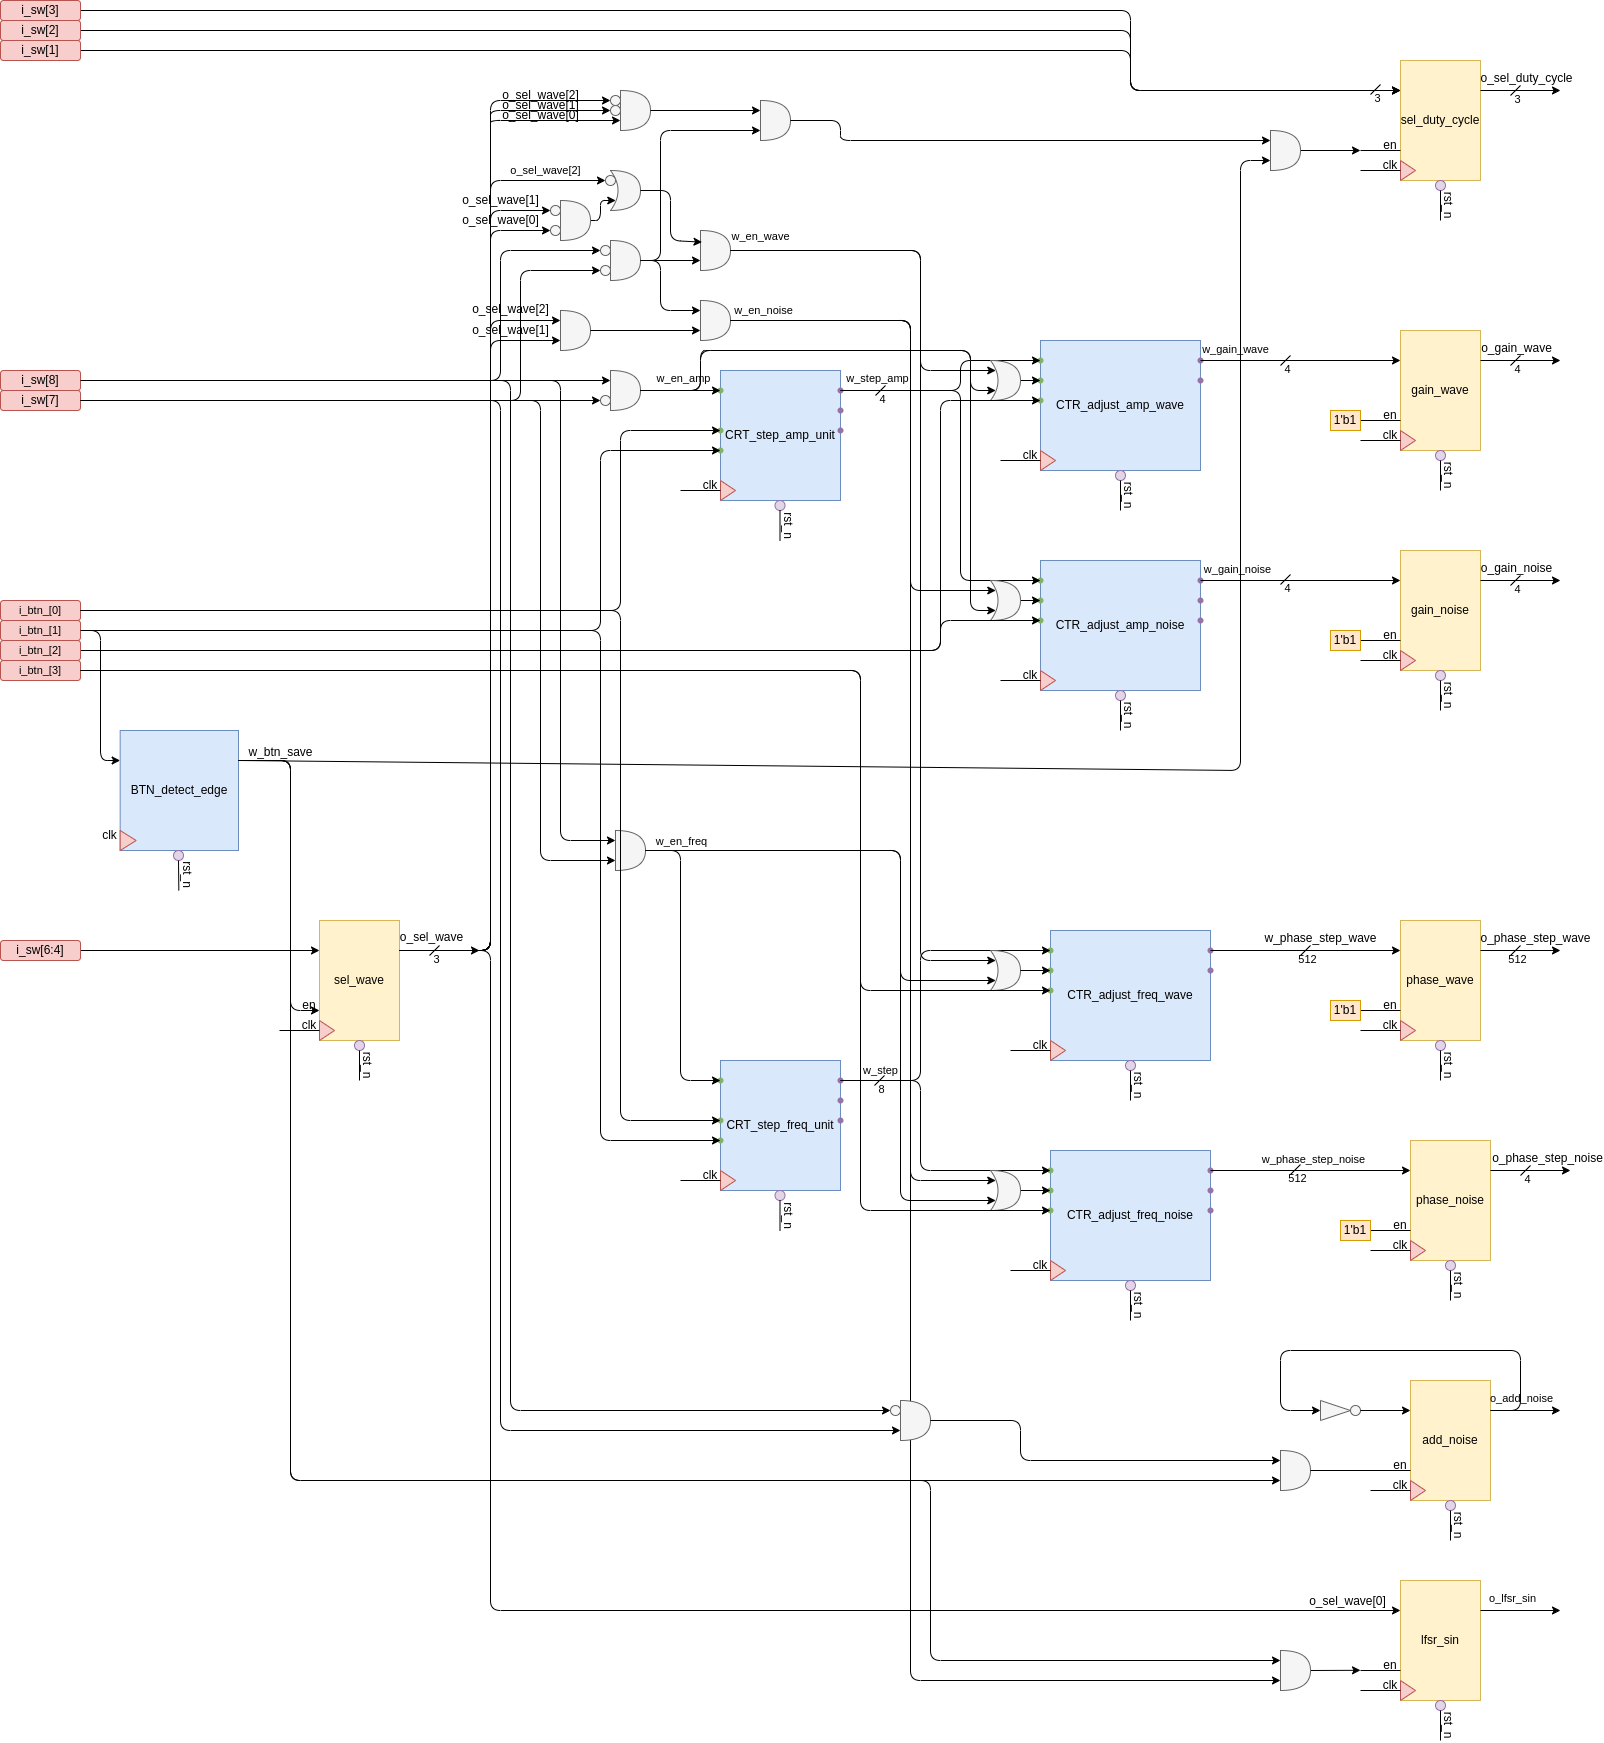
\includegraphics[width=.8\linewidth]{./../00_spec/spec/UI_rtl.png}
	\caption{Block diagram for Module Control value.}
\end{figure}


\section{Hardware Implementation Results}

\subsection{Simulation}

\subsubsection{Testbench}

\lstinputlisting[style=StyleCode ,language=SystemVerilog, caption={Testbench for Waveform Generator.}]{./../03_verif/wave_gen_tb.sv}

\subsubsection{Results of Wave Simulation}
\begin{figure}[H]
	\centering
	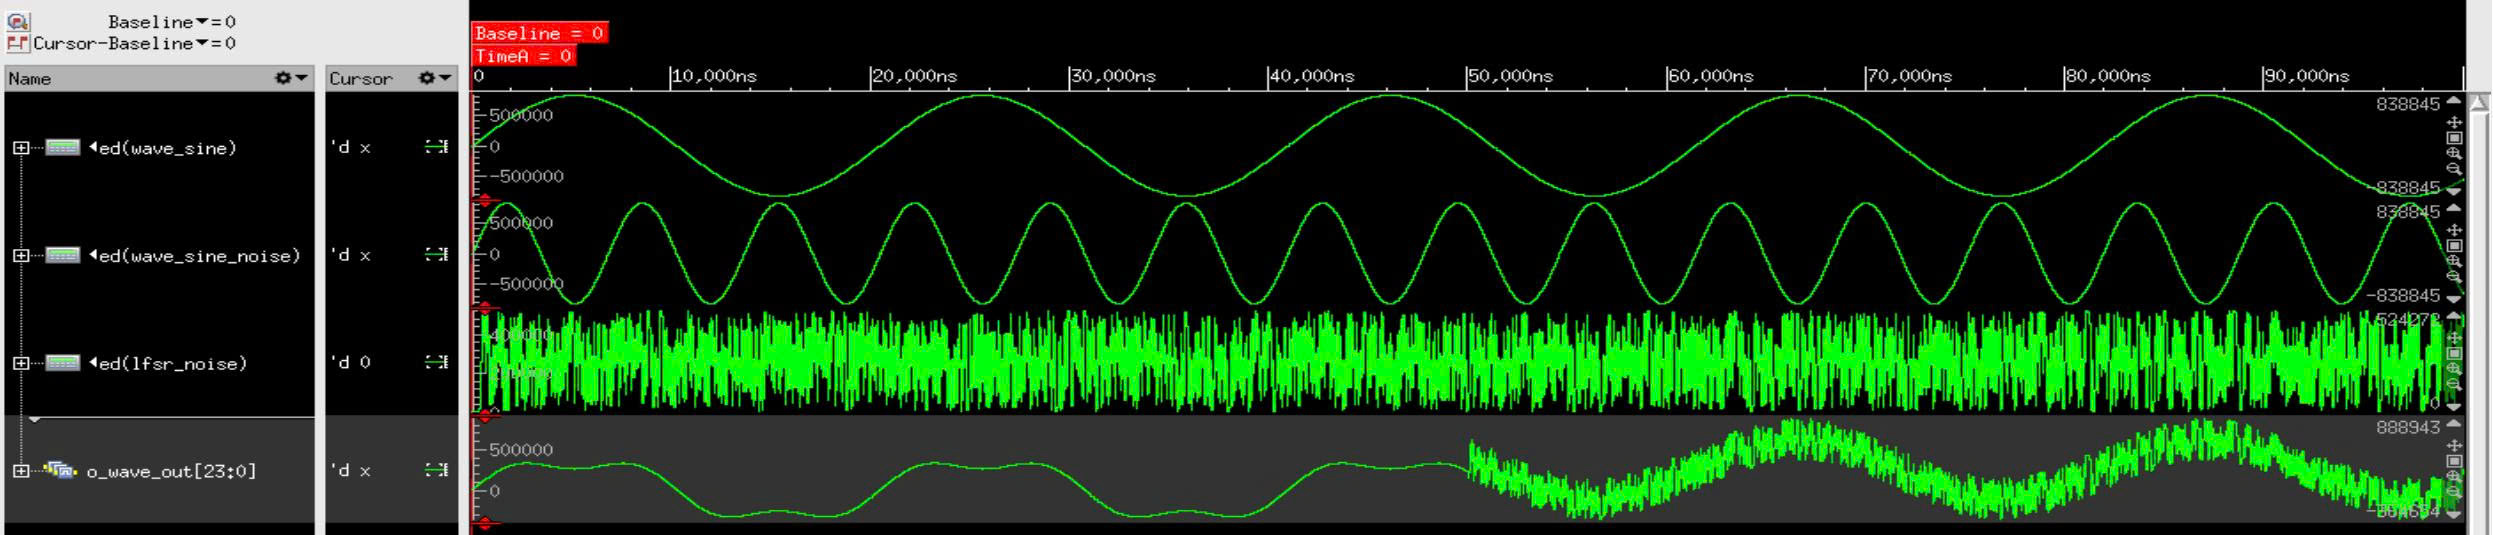
\includegraphics[width=.9\linewidth]{./my-chapters/my-images/simulation/sin_add_noise_sin.jpg}
	\caption{A sine wave affected by third-order harmonic sine noise and white noise.}
\end{figure}

\begin{figure}[H]
	\centering
	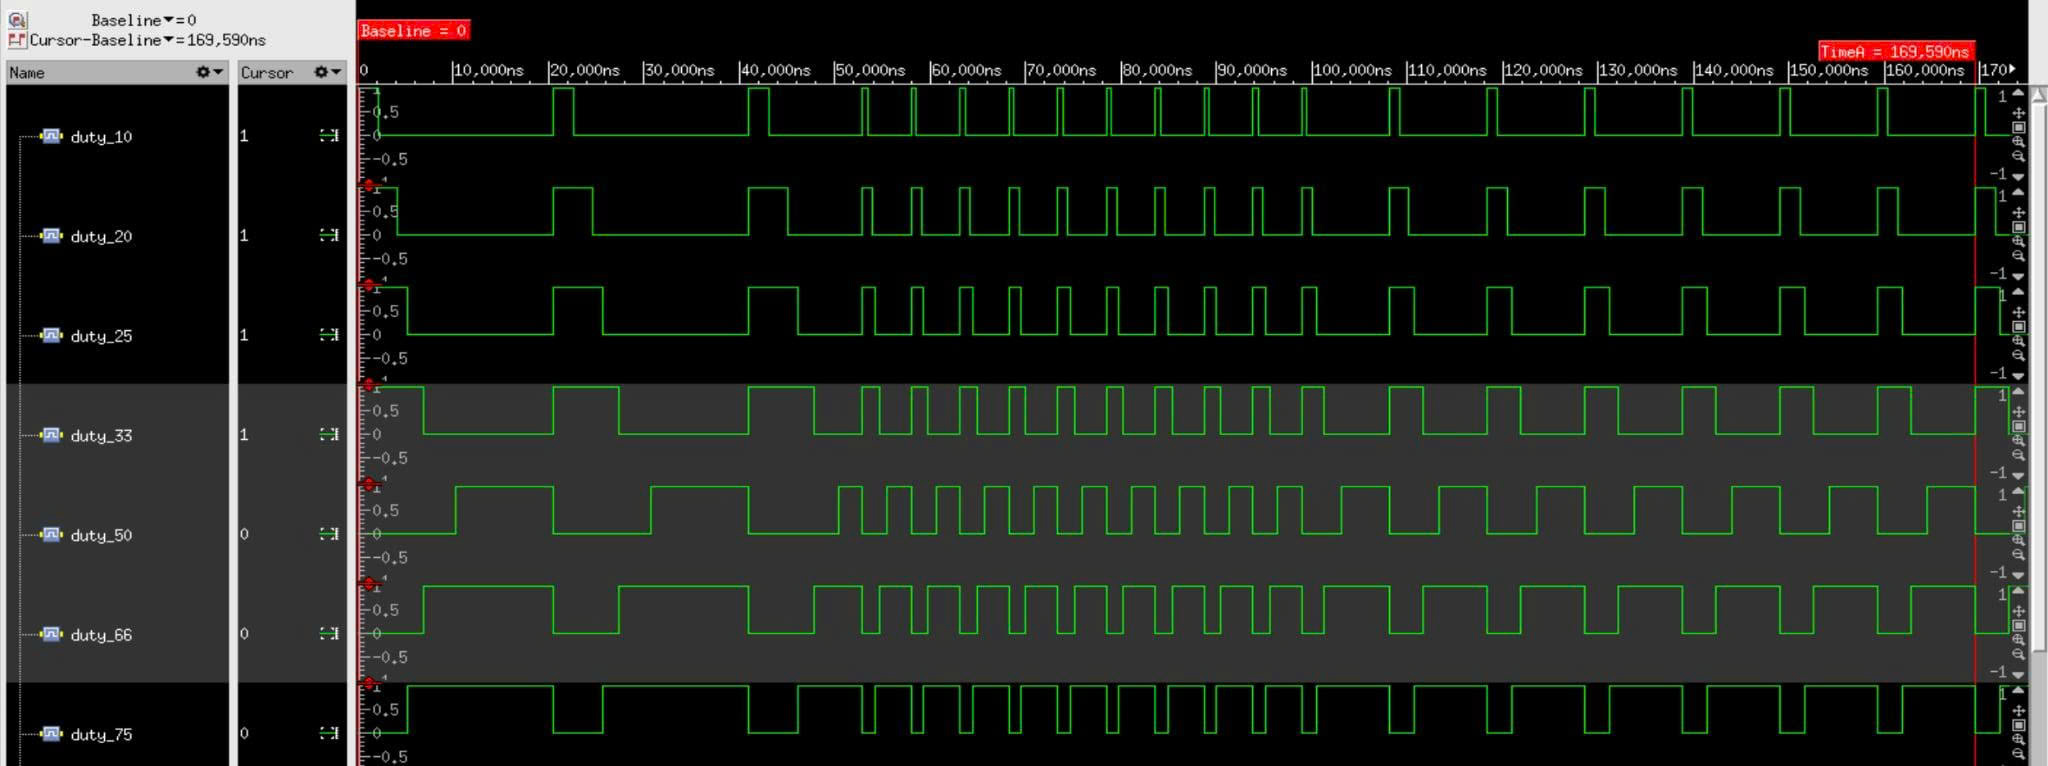
\includegraphics[width=.9\linewidth]{./my-chapters/my-images/simulation/duty_cycle.jpg}
	\caption{Demonstration of square waves with different duty cycles ranging from 10\% to 90\%.}
\end{figure}

\begin{figure}[H]
	\centering
	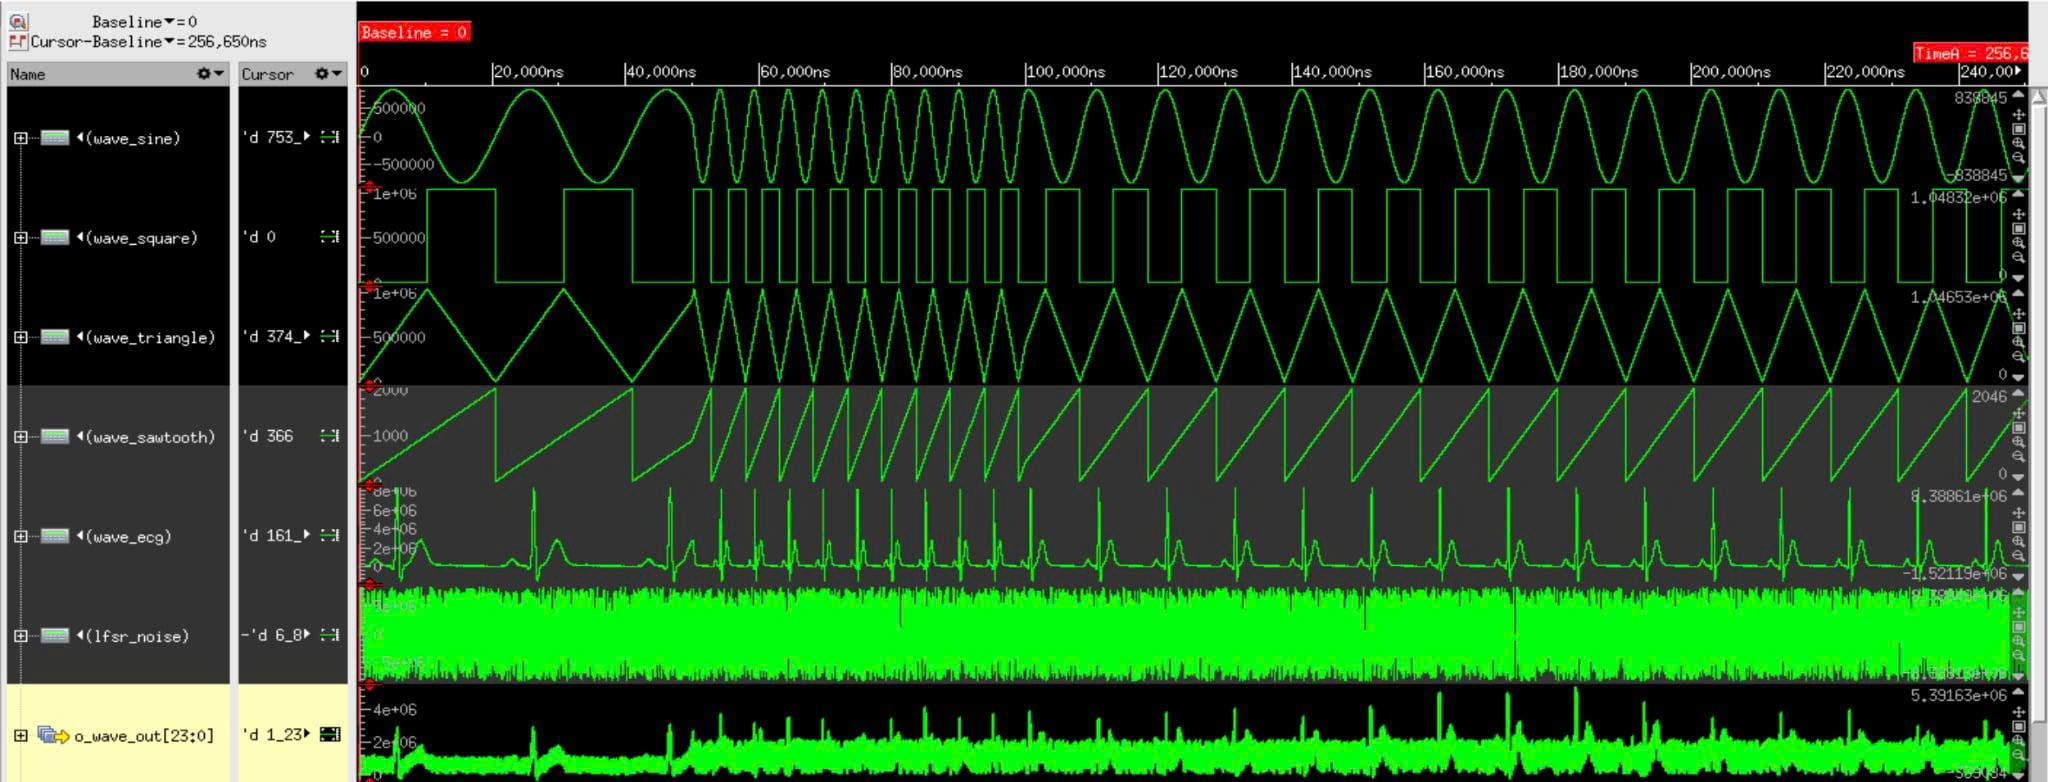
\includegraphics[width=.9\linewidth]{./my-chapters/my-images/simulation/waveform_with_noise.jpg}
	\caption{Basic waveforms and noise modulation: ECG output signal affected by frequency and amplitude variations of injected noise.}
\end{figure}

\subsection{Top module}

\begin{figure}[H]
	\centering
	\fbox{%
		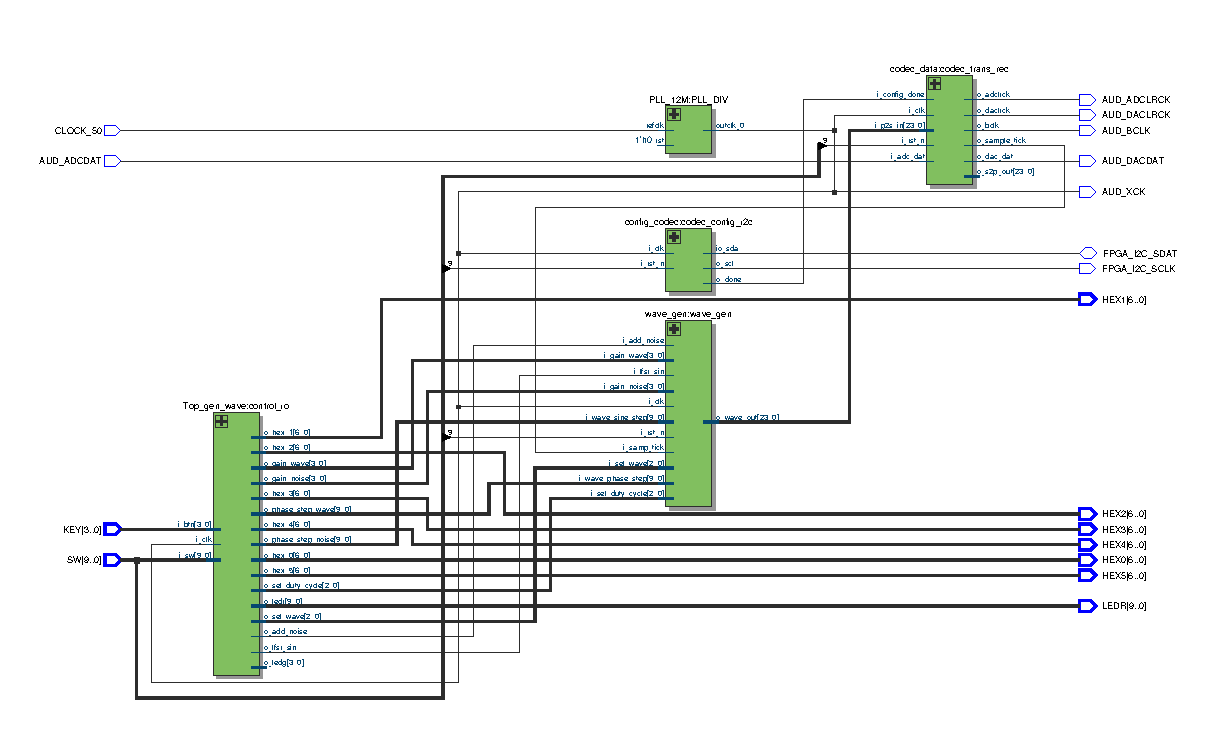
\includegraphics[width=\linewidth]{./my-chapters/my-diagrams/top_image.pdf}%
	}
	\caption{Block diagram for Top module.}
\end{figure}

\subsection{Measurement Waveform}

\begin{figure}[H]
	\centering
	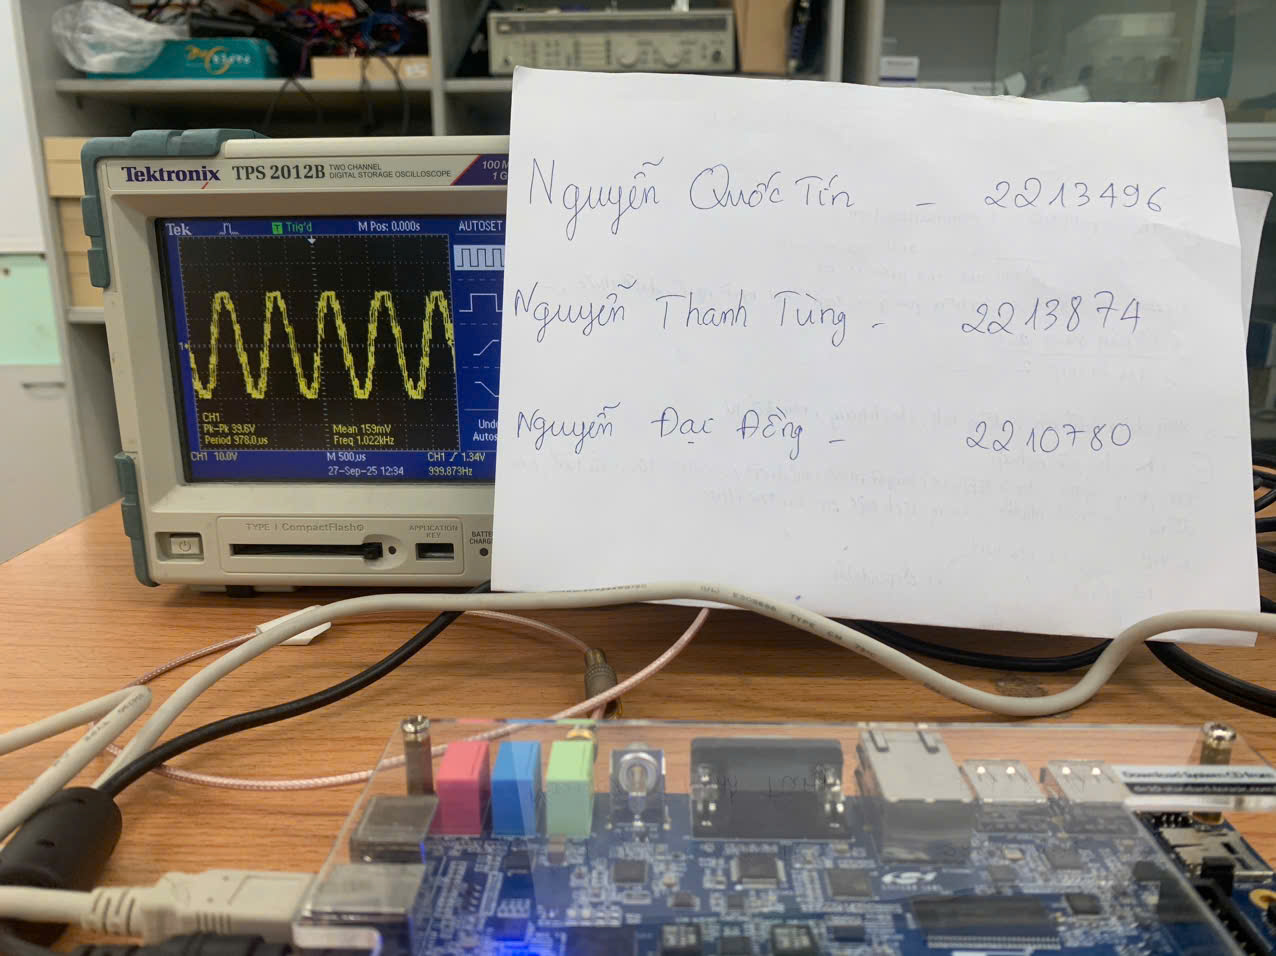
\includegraphics[width=.9\linewidth]{./my-chapters/my-images/Gen_wave/hinh2.jpg}
	\caption{Sine waveform on Oscilloscope.}
\end{figure}

\begin{figure}[H]
	\centering
	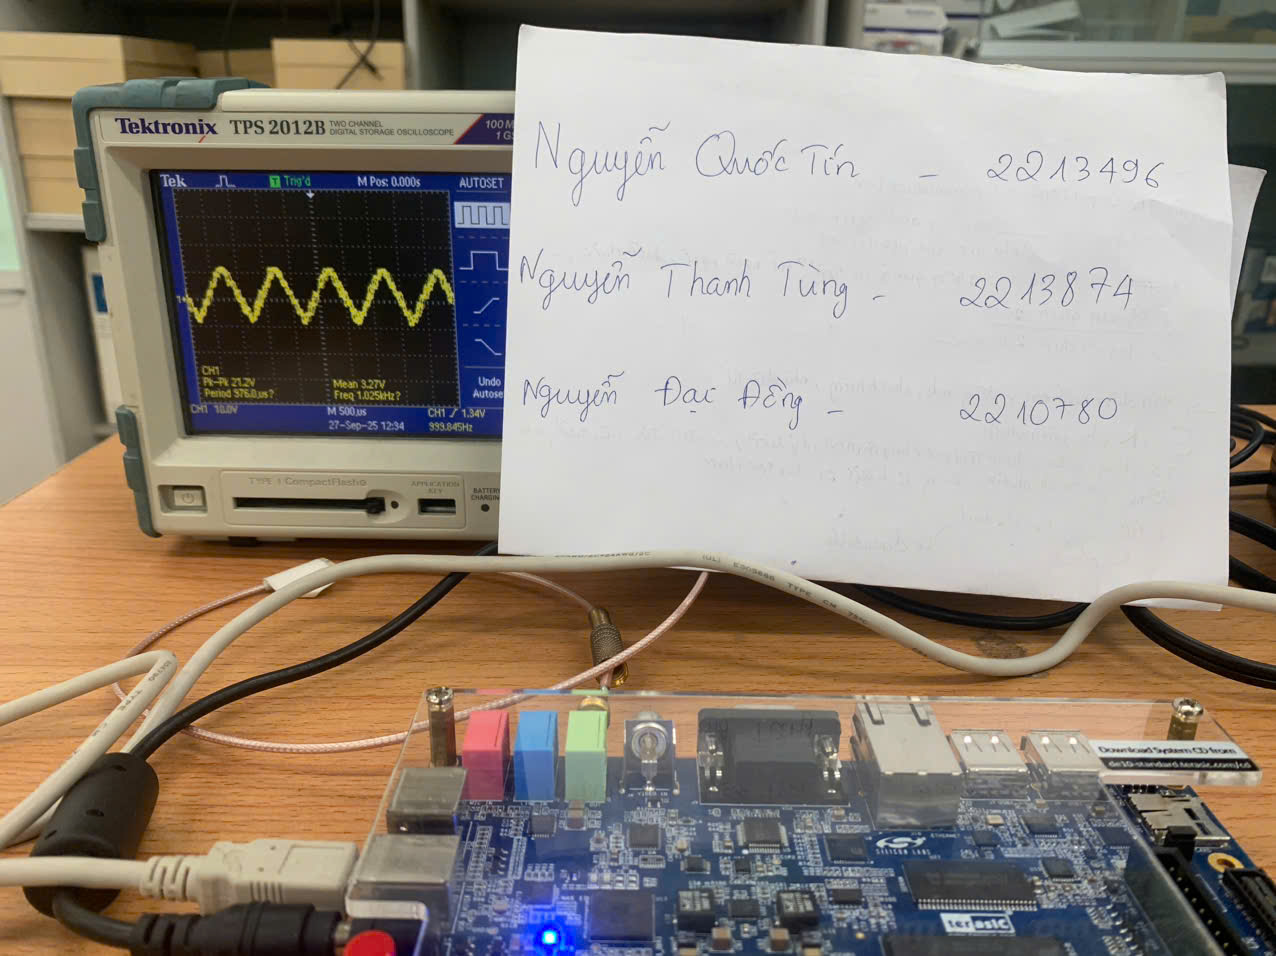
\includegraphics[width=.9\linewidth]{./my-chapters/my-images/Gen_wave/hinh5.jpg}
	\caption{Triangle waveform on Oscilloscope.}
\end{figure}

\begin{figure}[H]
	\centering
	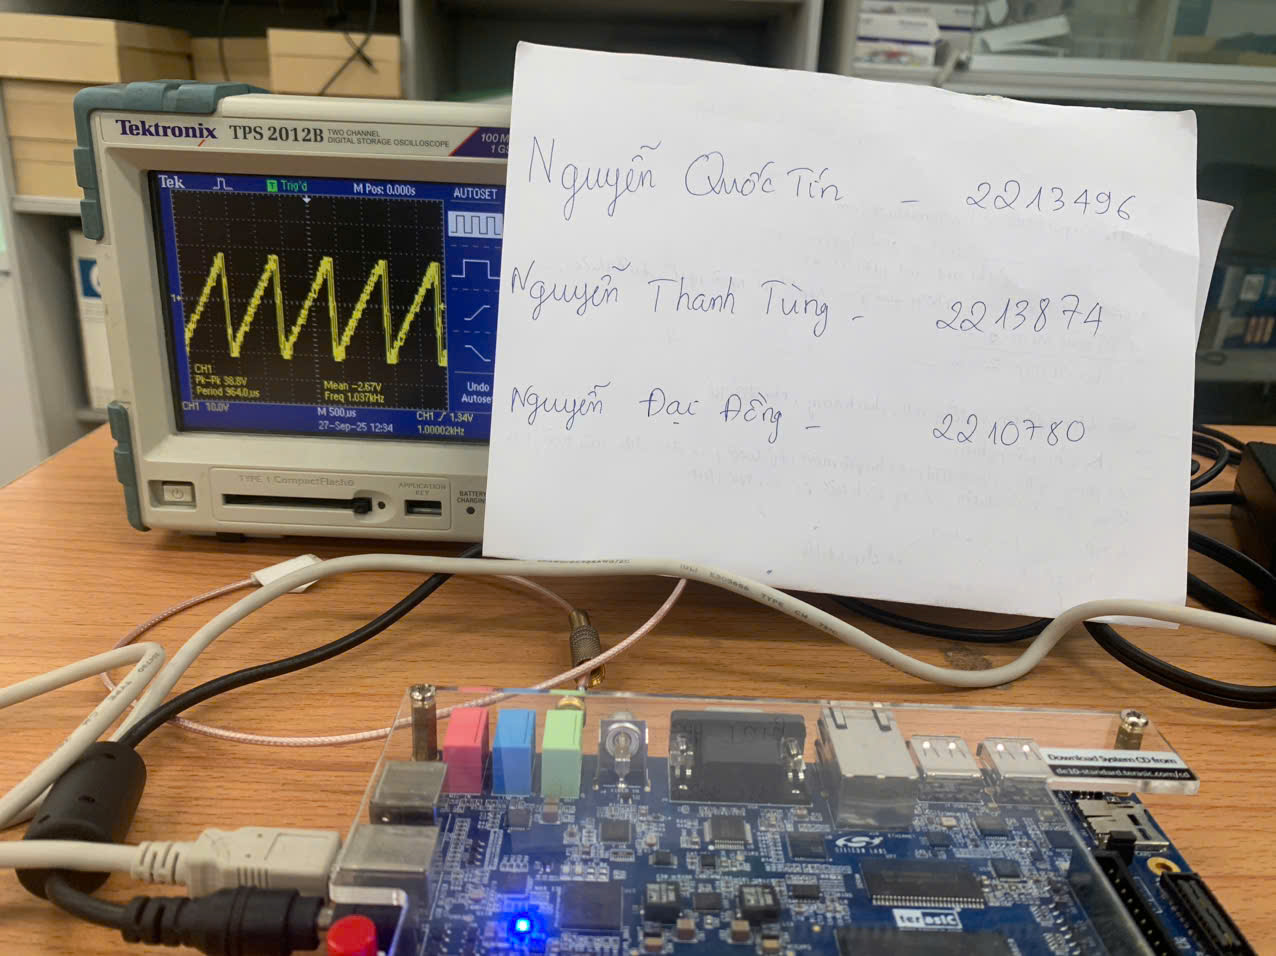
\includegraphics[width=.9\linewidth]{./my-chapters/my-images/Gen_wave/hinh4.jpg}
	\caption{Sawtooth waveform on Oscilloscope.}
\end{figure}

\begin{figure}[H]
	\centering
	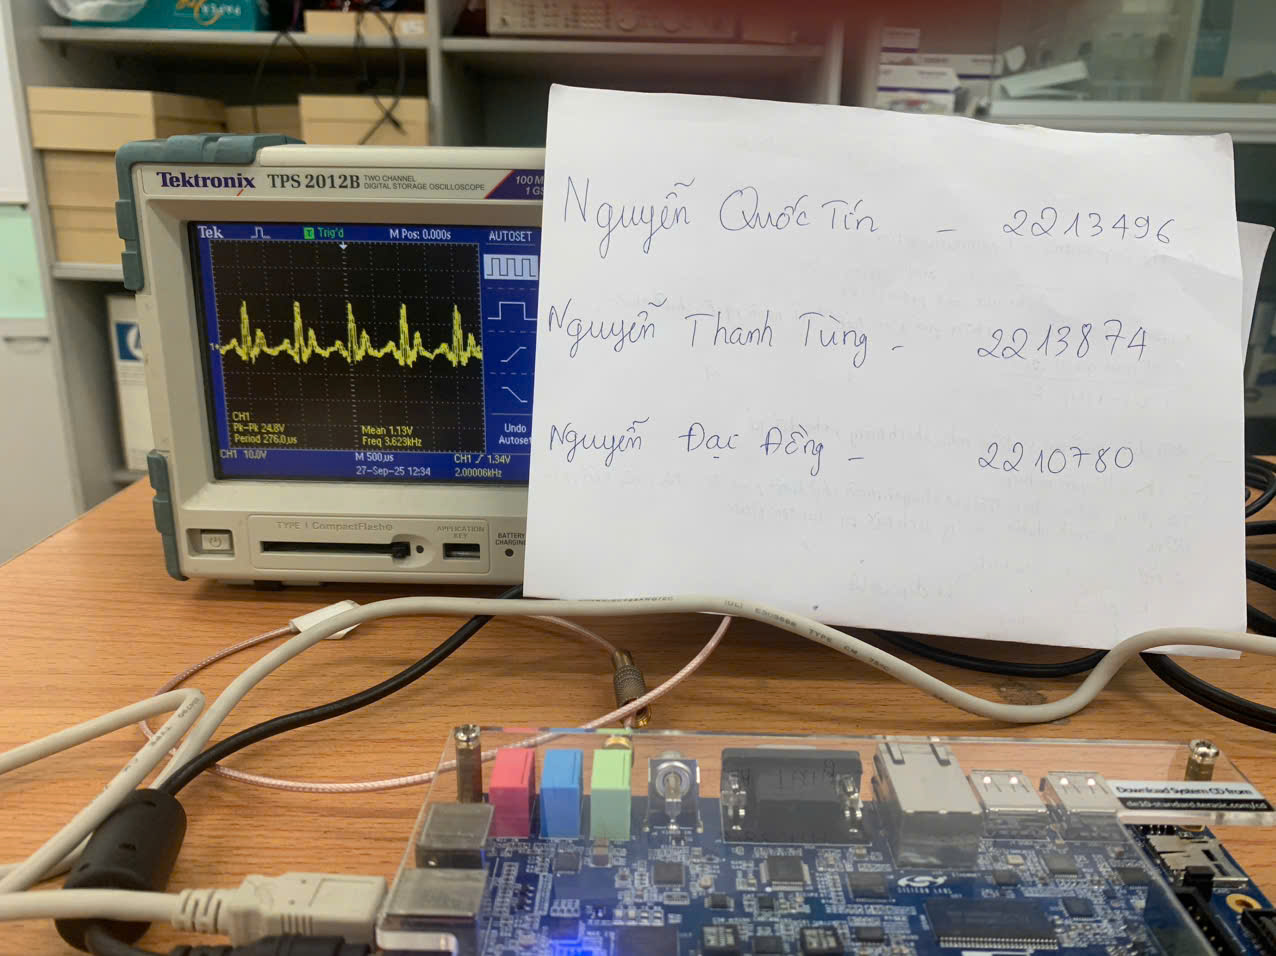
\includegraphics[width=.9\linewidth]{./my-chapters/my-images/Gen_wave/hinh3.jpg}
	\caption{ECG waveform on Oscilloscope.}
\end{figure}
\end{document}
